%% Rockable technical note: skin meshes of R-shapes.
%% Documentation of the geometric tools ShapeSDF / ShapeMesh / shape2mesh.
%% Build: make   (latexmk, then copies the PDF to ../skin-meshes.pdf,
%% the file offered for download by ../index.rst)
\documentclass[11pt,a4paper]{article}

\usepackage[T1]{fontenc}
\usepackage{newtxtext,newtxmath}
\usepackage[a4paper,margin=2.3cm,headheight=14pt]{geometry}
\usepackage{microtype}
\usepackage{amsmath}
\usepackage{graphicx}
\usepackage{booktabs}
\usepackage{tabularx}
\usepackage{algorithm}
\usepackage{algpseudocode}
\usepackage{tikz}
\usetikzlibrary{calc}
\usepackage{xcolor}
\usepackage[font=small,labelfont=bf]{caption}
\usepackage[numbers,sort&compress]{natbib}
\usepackage{fancyhdr}
\usepackage{enumitem}
\usepackage[colorlinks,linkcolor=black,citecolor=teal!70!black,urlcolor=teal!70!black]{hyperref}

% Common notation
\newcommand{\Rmink}{R}                 % Minkowski (rounding) radius
\newcommand{\skel}{\mathcal{K}}        % skeleton
\newcommand{\ball}{\mathcal{B}}        % ball
\newcommand{\shape}{\mathcal{S}}       % r-shape (solid)
\newcommand{\sdf}{f}                   % signed distance function
\newcommand{\norm}[1]{\left\lVert #1 \right\rVert}
\newcommand{\vect}[1]{\mathbf{#1}}
\newcommand{\sgnsdf}{\zeta}
\newcommand{\sag}{\epsilon}
\newcommand{\code}[1]{\texttt{#1}}

\definecolor{myTeal}{RGB}{0,166,164}
\setlength{\emergencystretch}{3em}

\pagestyle{fancy}
\fancyhf{}
\fancyhead[L]{\small\textsc{Rockable} --- Technical note}
\fancyhead[R]{\small Skin meshes of $R$-shapes}
\fancyfoot[C]{\small\thepage}
\renewcommand{\headrulewidth}{0.4pt}

\begin{document}

% ---------------------------------------------------------------- title block
\thispagestyle{plain}
\begin{center}
  {\small\textsc{Rockable documentation --- Technical note}}\\[10pt]
  {\LARGE\bfseries Watertight skin meshes of three-dimensional $R$-shapes:\\[3pt]
  exact distance, visualisation and mass properties\par}
  \vspace{12pt}
  {\large Vincent Richefeu}\\[4pt]
  {\small Laboratoire 3SR, Universit\'e Grenoble Alpes, CNRS, Grenoble INP,
  38000 Grenoble, France\\
  \href{mailto:vincent.richefeu@univ-grenoble-alpes.fr}{\nolinkurl{vincent.richefeu@univ-grenoble-alpes.fr}}}\\[6pt]
  {\small October 2026 \quad$\cdot$\quad Code: \url{https://github.com/richefeu/rockable}}
\end{center}

\vspace{4pt}
\begin{abstract}
\noindent
In \code{Rockable}, a grain is an $R$-shape (a sphero-polyhedron): the Minkowski
sum of a skeleton (vertices, edges and faces) and a ball of radius~$\Rmink$.
Only the skeleton and the radius are stored, so the surface of the grain is
never built, and the viewers draw overlapping spheres, tubes and plates instead.
This drawing fails with transparency and cannot be exported. This note documents
the tools added to \code{Rockable} to build the surface explicitly. They rely on
classical results of solid modelling and computer graphics, recalled with their
references: the signed distance to an $R$-shape is the signed distance to its
skeleton minus~$\Rmink$, exact everywhere, with an analytic gradient; marching
cubes on this function, followed by a Newton projection of each vertex onto the
exact surface, gives a watertight triangle mesh whose only error is the chordal
error set by one tolerance; a coplanar merge removes the extra triangles that
marching cubes leaves on flat faces; and the divergence theorem applied to the
mesh gives the volume, centre of mass and inertia tensor at second order in the
grid step. For each step, the note gives the corresponding classes, functions,
options and files of the code (\code{ShapeSDF}, \code{buildShapeMesh},
\code{simplifyCoplanar}, the \code{shape2mesh} tool and the \code{.rmsh} file read
by the viewers), the validation tests shipped with the code, and the known
limits.
\end{abstract}

\noindent\textbf{Keywords:} sphero-polyhedra; discrete element method; signed
distance function; offset surface; marching cubes; mass properties;
visualisation.

\vspace{6pt}
\noindent\fbox{\parbox{\dimexpr\linewidth-2\fboxsep-2\fboxrule}{\small
\textbf{In short.} \quad
\code{shape2mesh shapes.txt --rmsh -s} writes \code{shapes.rmsh} next to the shape
file; \code{see} then draws every particle with its watertight skin instead of the
overlapping primitives. \code{shape2mesh shapes.txt -f ply -e 1e-3} exports one
mesh per shape, with exact normals, for Blender, ParaView or MeshLab.
Section~\ref{sec:usage} gives the workflow, and Table~\ref{tab:codemap} maps each
section of this note to the code.}}

% =====================================================================
\section{Introduction}
\label{sec:intro}

The discrete-element method (DEM) models a granular medium as a set of rigid
grains and follows their motion under contact forces and body forces. Grain
shape controls packing, dilatancy, force transmission and strength, so its
description is a central part of a DEM model, and many descriptions coexist,
each with its own balance between geometric accuracy and contact
cost~\cite{lu2015}: clumps of glued spheres~\cite{favier1999}, polyhedra with
specific contact schemes~\cite{cundall1988}, superquadrics~\cite{podlozhnyuk2017},
potential particles~\cite{houlsby2009}, and level sets sampled on a grid, which
can be read directly from tomographic images of real
sand~\cite{kawamoto2016,kawamoto2018}.

\code{Rockable}~\cite{richefeu2025rockable} uses sphero-polyhedra, called
\emph{$R$-shapes} in the code: a base polyhedron rounded by a sphere of fixed
radius~$\Rmink$. This description, introduced in DEM by Pournin and
Liebling~\cite{pournin2005,pournin2009} and developed by Alonso-Marroqu\'in,
Galindo-Torres and co-workers~\cite{alonso2008,alonso2009,galindo2010}, keeps the
angular look of polyhedra while giving a well-defined normal everywhere, and it
reduces contact detection to distance queries between skeleton features, the
basic queries of collision detection~\cite{gilbert1988,vandenbergen2003,ericson2005}.
The reference article of \code{Rockable}~\cite{richefeu2025rockable} describes the
contact model, the time integration and the parallelisation. The code has been
used for rock avalanches and boulder
impacts~\cite{richefeu2012,mollon2012,mollon2015,garcia2020}, the compression of
brittle hollow particles~\cite{stasiak2022}, and the flow, elasticity and
fracture of polyhedral grains~\cite{vu2024drum,vu2024elast,vu2024frac}, and some of
its features were ported to ExaDEM~\cite{prat2025}.

\begin{figure}[t]
  \centering
  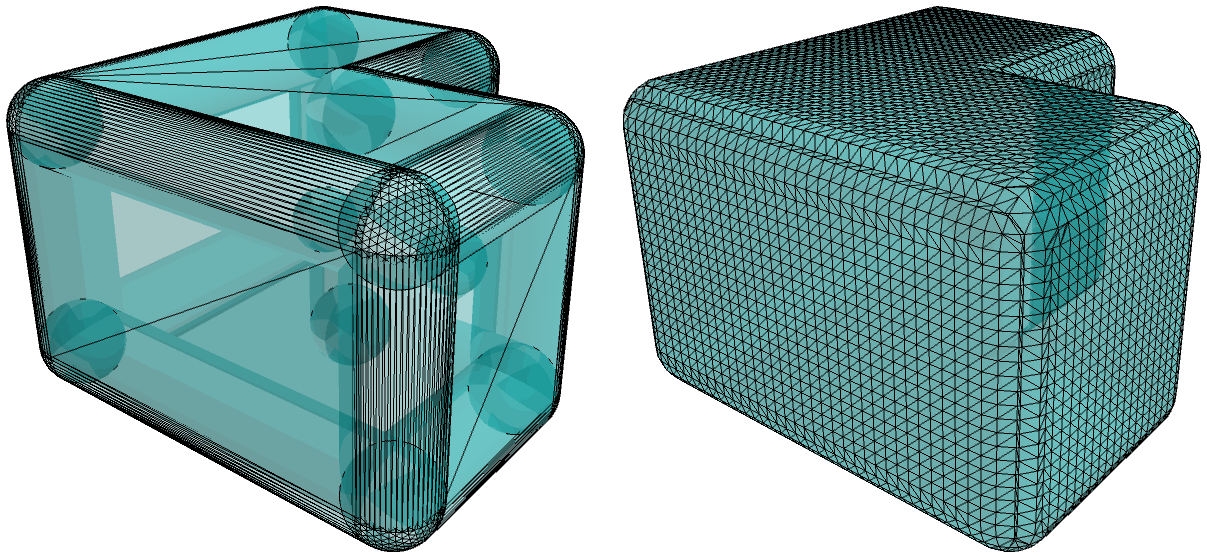
\includegraphics[width=0.8\linewidth]{figures/motivation}
  \caption{The same $R$-shape (an L-prism) shown semi-transparently in the
  \code{Rockable} viewer, from one camera. \emph{Left}: the overlapping
  primitives used for display: a sphere per vertex, a tube per edge and two
  offset polygons per face. When they are opaque, a depth buffer hides their
  interiors and they look like a solid. With transparency, every internal
  sphere, tube and face becomes visible, and the surfaces that coincide are
  blended several times. \emph{Right}: the single watertight skin mesh described
  in this note, which is one consistent translucent solid. Both panels are
  rendered by the same viewer.}
  \label{fig:motivation}
\end{figure}

This note is about visualisation, where the Minkowski-sum structure of an
$R$-shape had not been used in \code{Rockable}. An $R$-shape is stored only as a
skeleton and a radius, so its surface is never built explicitly. The viewers
(\code{see}, \code{shapeSurvey}) approximate it with a set of overlapping
primitives: one sphere per vertex, one tube per edge, and two offset polygons per
face. This set is not a single closed surface but a group of overlapping solids.
In an opaque image a depth buffer hides this; with transparency the separate
primitives become visible (Figures~\ref{fig:motivation}
and~\ref{fig:transparency-bunny}), and the union can neither be lit with shadows
nor exported to a standard mesh format.

What is missing is an explicit, watertight surface. The Minkowski sum gives it
directly: the surface of an $R$-shape is the offset surface of its skeleton at
distance~$\Rmink$, a classical object of solid
modelling~\cite{rossignac1986}, and its signed distance is the signed distance to
the skeleton minus~$\Rmink$. None of the ingredients used below is new; they are
recalled in Section~\ref{sec:related} with their references. The purpose of this
note is to document how they are combined in \code{Rockable}, which choices were
made and why, how the result was validated, and where its limits are.

\begin{figure}[t]
  \centering
  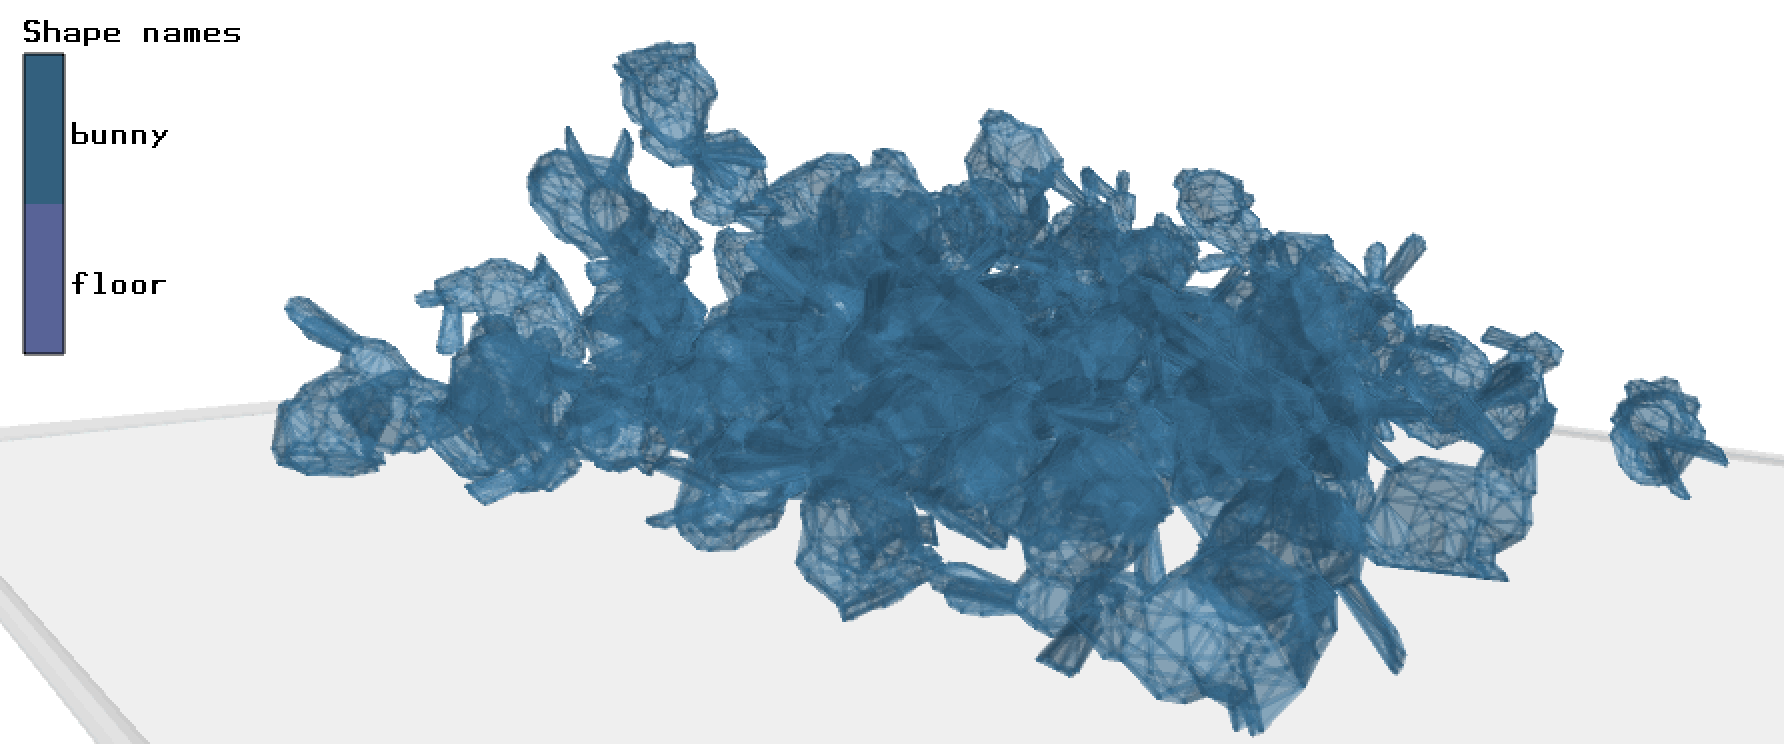
\includegraphics[width=0.8\linewidth]{figures/without-skin}\\[2pt]
  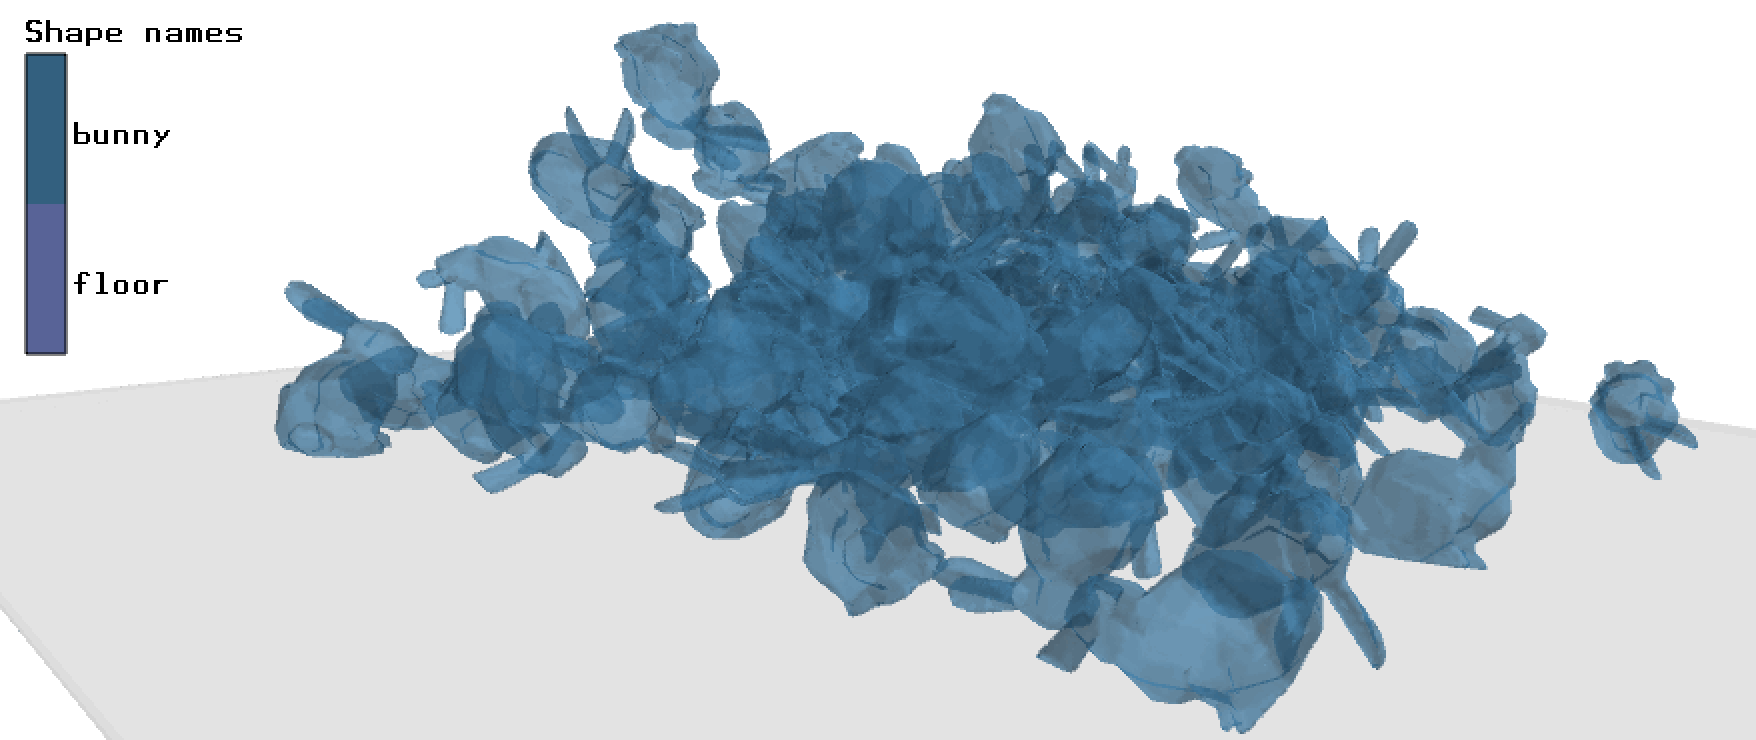
\includegraphics[width=0.8\linewidth]{figures/with-skin}
  \caption{About one hundred Stanford bunnies falling to form a heap, shown
  semi-transparently in \code{see}. Top: the overlapping-primitive drawing; the
  seams and the internal facets of the primitives fill the image. Bottom: the
  same scene drawn with the skin meshes read from the \code{.rmsh} companion
  file (Section~\ref{sec:usage}).}
  \label{fig:transparency-bunny}
\end{figure}

The note is organised as follows. Section~\ref{sec:related} reviews the related
work. Section~\ref{sec:rshapes} recalls the $R$-shape model of \code{Rockable}.
Section~\ref{sec:sdf} gives the signed distance function and its sign rules
(class \code{ShapeSDF}), Section~\ref{sec:meshing} the mesher
(\code{buildShapeMesh}), Section~\ref{sec:simplify} the coplanar merge
(\code{simplifyCoplanar}), and Section~\ref{sec:mass} the mass properties by the
divergence theorem. Section~\ref{sec:usage} describes the tools and files seen by
the user, Section~\ref{sec:results} the validation, and Section~\ref{sec:complex}
stress tests on difficult skeletons, with the cases where the mesher fails.

% =====================================================================
\section{Related work}
\label{sec:related}

\paragraph{Offset surfaces and Minkowski sums}
The solid obtained by moving a ball of radius $\Rmink$ over a set is its
\emph{offset}, or Minkowski sum with the ball. Rossignac and
Requicha~\cite{rossignac1986} gave the mathematical properties of solid offsetting
and noted, among others, that offsetting rounds convex features and keeps concave
ones sharp, which is the behaviour described in Section~\ref{sec:rshapes}. Exact
Minkowski sums of polyhedra are combinatorially expensive, which led to
approximate, volumetric constructions~\cite{varadhan2006}. Closest to the present
tools, Pavi\'c and Kobbelt~\cite{pavic2008} compute the offset of a triangle mesh
as the union of spheres, cylinders and prisms, by evaluating a distance on a
volumetric grid and extracting its iso-surface; their unsigned distance tolerates
non-manifold input, an issue also met below. For convex bodies, Steiner's formula
gives the volume of the offset as a polynomial in~$\Rmink$~\cite{schneider2014},
which provides closed-form reference volumes for convex $R$-shapes.

\paragraph{Distance fields}
Signed distance fields are a standard representation of shape in graphics; the
survey of Jones et al.~\cite{jones2006} covers their computation and use, and
adaptive sampling~\cite{frisken2000} reduces their storage. Computing the sign of
the distance to a triangle mesh is the delicate part. The angle-weighted
pseudonormal of B{\ae}rentzen and Aan{\ae}s~\cite{baerentzen2005} gives an exact
sign for a closed manifold; ray casting with a parity
count~\cite{orourke1998,moller1997} tolerates small defects; the generalized
winding number~\cite{jacobson2013} is robust to open and self-intersecting meshes.
An $R$-shape is a case where the distance is \emph{exact} and cheap, because it
reduces to point--primitive queries on the
skeleton~\cite{vandenbergen2003,ericson2005}, accelerated by a bounding-volume
hierarchy~\cite{vandenbergen1997}. Such a function can also be rendered without
any mesh by sphere tracing~\cite{hart1996}; a mesh was preferred here because it
is reused for export and for the mass properties.

\paragraph{Polygonization of implicit surfaces}
Marching cubes~\cite{lorensen1987} and its many variants~\cite{newman2006},
including the treatment of ambiguous cases~\cite{nielson1991,lewiner2003}, and
earlier polygonizers of implicit surfaces~\cite{bloomenthal1988}, extract a
triangle mesh from a sampled scalar field. Projecting the vertices onto the exact
iso-surface with the gradient is a common refinement when the function is known
analytically. Marching cubes rounds sharp creases; the extended marching cubes of
Kobbelt et al.~\cite{kobbelt2001} and dual contouring~\cite{ju2002} recover them
from Hermite data (positions and normals), which the present mesher already
stores. A general reference on these operations is the book of Botsch et
al.~\cite{botsch2010}.

\paragraph{Mesh simplification}
Merging the coplanar triangles produced by an iso-surface extractor and
re-triangulating the merged polygons was proposed by Hinker and
Hansen~\cite{hinker1993}; superfaces~\cite{kalvin1996} grow nearly planar regions
under a bounded error, and vertex decimation~\cite{schroeder1992} removes vertices
and re-triangulates the hole. More general methods, such as edge collapse with a
quadric error metric~\cite{garland1997}, trade a controlled error for a target
size. The re-triangulation uses ear clipping~\cite{meisters1975,orourke1998},
whose robust implementation on degenerate polygons is discussed by
Held~\cite{held2001}.

\paragraph{Mass properties}
The volume, first and second moments of a polyhedron follow from the divergence
theorem as sums over its faces~\cite{lien1984,mirtich1996}. For a triangle mesh,
the sums reduce to closed-form tetrahedron integrals~\cite{tonon2005,kallay2006}.
The alternative used so far in \code{Rockable} is quasi-Monte-Carlo integration
with a Sobol sequence~\cite{sobol1967,niederreiter1992}; its convergence is slowed
by the discontinuity of the integrand at the
surface~\cite{he2015}, an effect measured in Section~\ref{sec:mass}.

\paragraph{What is specific here}
The tools documented below are a direct assembly of these methods. What the
$R$-shape model brings is that the distance is exact everywhere and its smallest
radius of curvature is known ($\Rmink$), so that a single tolerance fixes the grid
step, the offset faces are exact planes that can be merged without error, and the
mesh depends only on the shape, so it is computed once and shared by all the
particles that use it.

% =====================================================================
\section{Sphero-polyhedral shapes in Rockable}
\label{sec:rshapes}

An $R$-shape is defined by a \emph{skeleton} and a rounding radius. In a
\code{Rockable} shape file, each shape is a block that gives its \code{name}, its
\code{radius}~$\Rmink$, and the skeleton in the body frame: \code{nv} vertices,
\code{ne} edges (pairs of vertex indices) and \code{nf} faces (planar polygons);
the keyword \code{isSurface} declares that the faces form an open surface rather
than the boundary of a solid. In memory, this is the class \code{Shape}
(\code{src/Core/Shape.hpp}). The $R$-shape is the set
%
\begin{equation}
  \shape = \{\, \vect{x} : \sgnsdf(\vect{x})\operatorname{dist}(\vect{x},\skel) \le \Rmink \,\},
  \label{eq:minkowski}
\end{equation}
%
where the sign $\sgnsdf(\vect{x})$ is $-1$ when $\vect{x}$ lies in a volume
enclosed by the faces of the skeleton and $+1$ everywhere else. Every point within
a distance $\Rmink$ of the skeleton belongs to the shape, and so does every point
of the volume enclosed by its faces. Geometrically, $\shape$ is the Minkowski sum
of the filled skeleton and the ball $\ball(\Rmink)$. A skeleton that encloses no
volume (a point, a segment, an open plate) has $\sgnsdf\equiv+1$, and the shape is
a ball, a capsule or a slab.

The figures of this section are drawn in two dimensions, where the skeleton has
only vertices and edges and the $R$-shape is a
\emph{sphero-polygon}~\cite{alonso2008} (Figure~\ref{fig:construction}). The 3D
case adds planar faces, whose offset gives flat surface patches.

The distance from a point $\vect{x}$ to the skeleton is the smallest distance to
any primitive,
%
\begin{equation}
  \operatorname{dist}(\vect{x},\skel) = \min_{k\in\skel}\operatorname{dist}(\vect{x},k).
  \label{eq:distmin}
\end{equation}
%
The distance to a vertex is a point distance, to an edge a segment distance, and
to a face the distance to a planar polygon: the perpendicular distance if the foot
of the perpendicular lies inside the polygon, the distance to its boundary
otherwise~\cite{ericson2005}.

\begin{figure}[tb]
  \centering
  \begin{minipage}{0.48\linewidth}
  \centering
  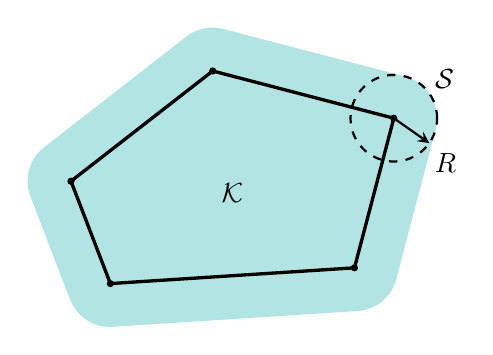
\begin{tikzpicture}[x=1cm,y=1cm,>=stealth]
    \pgfmathsetmacro{\Rval}{0.55}
    \pgfmathsetmacro{\Dval}{2*\Rval}
    \coordinate (A) at (0,0);
    \coordinate (B) at (3.1,0.2);
    \coordinate (C) at (3.6,2.1);
    \coordinate (D) at (1.3,2.7);
    \coordinate (E) at (-0.5,1.3);
    \fill[myTeal!30] (A)--(B)--(C)--(D)--(E)--cycle;
    \draw[myTeal!30,line width=\Dval cm,line cap=round,line join=round]
          (A)--(B)--(C)--(D)--(E)--cycle;
    \draw[very thick] (A)--(B)--(C)--(D)--(E)--cycle;
    \foreach \p in {A,B,C,D,E}{\fill (\p) circle (1.3pt);}
    \draw[dashed,thick] (C) circle (\Rval cm);
    \draw[->,thick] (C) -- ($(C)+(-35:\Rval)$);
    \node at ($(C)+(-30:{\Rval+0.15})+(0.05,-0.22)$) {$\Rmink$};
    \node at (1.55,1.15) {$\skel$};
    \node[anchor=west] at (4.0,2.6) {$\shape$};
  \end{tikzpicture}
  \caption{Construction of a sphero-polygon (2D). The skeleton $\skel$ (bold) is
  dilated by a disk of radius $\Rmink$ (dashed) into the solid $\shape$
  (shaded).}
  \label{fig:construction}
  \end{minipage}\hfill
  \begin{minipage}{0.48\linewidth}
  \centering
  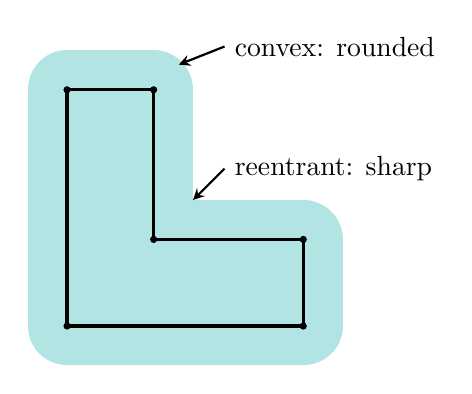
\begin{tikzpicture}[x=1cm,y=1cm,>=stealth]
    \pgfmathsetmacro{\Rval}{0.5}
    \pgfmathsetmacro{\Dval}{2*\Rval}
    \coordinate (P0) at (0,0);
    \coordinate (P1) at (3,0);
    \coordinate (P2) at (3,1.1);
    \coordinate (P3) at (1.1,1.1);
    \coordinate (P4) at (1.1,3);
    \coordinate (P5) at (0,3);
    \fill[myTeal!30] (P0)--(P1)--(P2)--(P3)--(P4)--(P5)--cycle;
    \draw[myTeal!30,line width=\Dval cm,line cap=round,line join=round]
          (P0)--(P1)--(P2)--(P3)--(P4)--(P5)--cycle;
    \draw[very thick] (P0)--(P1)--(P2)--(P3)--(P4)--(P5)--cycle;
    \foreach \p in {P0,P1,P2,P3,P4,P5}{\fill (\p) circle (1.3pt);}
    \draw[->,thick] (P4)+(0.9,0.55) node[anchor=west]{convex: rounded} -- ($(P4)+(0.32,0.32)$);
    \draw[->,thick] (P3)+(0.9,0.9) node[anchor=west]{reentrant: sharp} -- ($(P3)+(0.5,0.5)$);
  \end{tikzpicture}
  \caption{Convex versus reentrant features (2D). Convex corners are rounded with
  radius $\Rmink$; at the reentrant corner the dilation fills the notch and leaves
  a sharp crease.}
  \label{fig:reentrant}
  \end{minipage}
\end{figure}

The boundary of a convex $R$-shape is made of three kinds of patch: each face
gives a flat patch, parallel to the face and moved out by $\Rmink$; each convex
edge a cylindrical patch of radius $\Rmink$ over the outer dihedral angle; each
convex vertex a spherical patch of radius $\Rmink$. For such a shape, Steiner's
formula~\cite{schneider2014} gives the volume in closed form,
%
\begin{equation}
  V(\shape) = V(\skel) + A(\skel)\,\Rmink
            + \frac{\Rmink^2}{2}\sum_{e}\ell_e\,(\pi-\theta_e)
            + \frac{4}{3}\pi\Rmink^3,
  \label{eq:steiner}
\end{equation}
%
with $A(\skel)$ the area of the faces, $\ell_e$ the length of edge $e$ and
$\theta_e$ its interior dihedral angle. Only convex parts are rounded: at a
\emph{reentrant} edge or vertex, the dilation fills the notch and the surface keeps
a sharp crease (Figure~\ref{fig:reentrant})~\cite{rossignac1986}, and
Equation~(\ref{eq:steiner}) no longer holds. This is where a numerical method is
needed, and the crease also matters for meshing (Section~\ref{sec:meshing}).

Finally, the dimension of the skeleton sets the type of $R$-shape: a single
vertex gives a sphere, vertices and edges with no face give a union of capsules,
faces that enclose a volume give the usual sphero-polyhedron, and faces that form
an open surface give a slab of thickness $2\Rmink$. All these cases come from the
same Equation~(\ref{eq:minkowski}); only the sign $\sgnsdf$
(Section~\ref{sec:sign}) distinguishes a filled interior from a shell.

% =====================================================================
\section{Signed distance function (\texttt{ShapeSDF})}
\label{sec:sdf}

With Equation~(\ref{eq:minkowski}), an $R$-shape is an implicit solid. Its signed
distance function (SDF) is
%
\begin{equation}
  \sdf(\vect{x}) = s(\vect{x}) - \Rmink,
  \qquad s(\vect{x}) = \sgnsdf(\vect{x})\operatorname{dist}(\vect{x},\,\skel),
  \label{eq:sdf}
\end{equation}
%
where $s$ is the signed distance to the skeleton. Unlike the overlapping
primitives used for rendering, Equation~(\ref{eq:sdf}) is exact everywhere in
space, and $\norm{\nabla\sdf}=1$ wherever $\sdf$ is differentiable. The surface of
the $R$-shape is the zero level set $\{\sdf=0\}$. Since $s$ is the distance to a
fixed set, its gradient points from the closest skeleton point
$\vect{p}^\ast(\vect{x})$ towards $\vect{x}$,
%
\begin{equation}
  \nabla \sdf(\vect{x}) = \sgnsdf(\vect{x})\,
    \frac{\vect{x}-\vect{p}^\ast(\vect{x})}{\norm{\vect{x}-\vect{p}^\ast(\vect{x})}}.
  \label{eq:grad}
\end{equation}
%
The exact outward normal at a surface point is thus given by the same
closest-point query that gives the distance. The gradient is undefined only on the
skeleton itself, which lies at a distance $\Rmink$ inside the surface when
$\Rmink>0$. Since $\sdf$ is a true distance, the Newton step
%
\begin{equation}
  \vect{x} \leftarrow \vect{x} - \sdf(\vect{x})\,\nabla\sdf(\vect{x})
  \label{eq:newton}
\end{equation}
%
moves a point almost onto the surface in one iteration; it is used to project the
mesh vertices.

\paragraph{In the code} The class \code{ShapeSDF}
(\code{src/Core/ShapeSDF.hpp}) is built once from a \code{Shape}. Its methods
\code{closestPoint(x)} (distance, closest point, and type and index of the
primitive), \code{value(x)} (Equation~\ref{eq:sdf}), \code{gradient(x)}
(Equation~\ref{eq:grad}) and \code{inside(x)} answer the queries. The
closest-point query is the minimum of Equation~(\ref{eq:distmin}); computed
directly it costs $\mathcal{O}(|\skel|)$, so it goes through an axis-aligned
bounding-box tree built by recursive median
split~\cite{vandenbergen1997,vandenbergen2003}. Two trees are built: one over all
primitives (closest point) and one over the faces only (sign).

\subsection{Determining the sign}
\label{sec:sign}

\begin{figure}[tb]
  \centering
  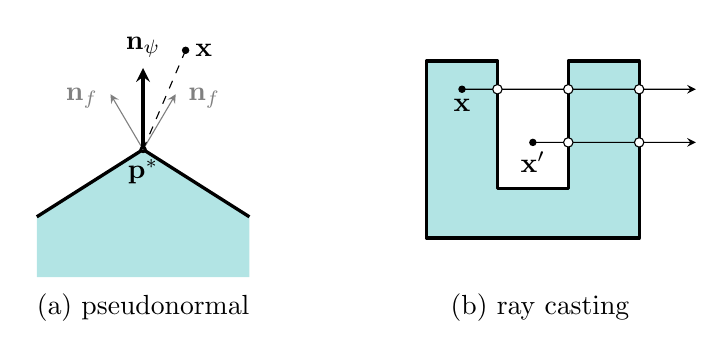
\begin{tikzpicture}[x=1cm,y=1cm,>=stealth,scale=0.9]
    \begin{scope}
      \coordinate (v) at (0,0);
      \coordinate (ea) at (-1.5,-0.95);
      \coordinate (eb) at (1.5,-0.95);
      \fill[myTeal!30] (ea)--(v)--(eb)--(1.5,-1.8)--(-1.5,-1.8)--cycle;
      \draw[very thick] (ea)--(v)--(eb);
      \fill (v) circle (1.5pt);
      \node[anchor=north] at (v) {$\vect{p}^\ast$};
      \draw[->,gray] (v) -- ($(v)+(-0.46,0.78)$);
      \draw[->,gray] (v) -- ($(v)+(0.46,0.78)$);
      \node[gray,anchor=east] at ($(v)+(-0.5,0.72)$) {$\vect{n}_f$};
      \node[gray,anchor=west] at ($(v)+(0.5,0.72)$) {$\vect{n}_f$};
      \draw[->,very thick] (v) -- (0,1.15) node[anchor=south] {$\vect{n}_\psi$};
      \coordinate (x) at (0.6,1.4);
      \fill (x) circle (1.5pt); \node[anchor=west] at (x) {$\vect{x}$};
      \draw[dashed] (v) -- (x);
      \node[anchor=north] at (0,-1.9) {(a) pseudonormal};
    \end{scope}
    \begin{scope}[xshift=5.5cm]
      \def\Upath{(-1.5,-1.25) -- (1.5,-1.25) -- (1.5,1.25) -- (0.5,1.25)
                 -- (0.5,-0.55) -- (-0.5,-0.55) -- (-0.5,1.25) -- (-1.5,1.25) -- cycle}
      \fill[myTeal!30] \Upath;
      \draw[very thick,line join=round] \Upath;
      \coordinate (xi) at (-1.0,0.85);
      \draw[->] (xi) -- (2.3,0.85);
      \foreach \xc in {-0.5,0.5,1.5}{\fill[white,draw=black] (\xc,0.85) circle (1.9pt);}
      \fill (xi) circle (1.5pt); \node[anchor=north] at (xi) {$\vect{x}$};
      \coordinate (xo) at (0.0,0.1);
      \draw[->] (xo) -- (2.3,0.1);
      \foreach \xc in {0.5,1.5}{\fill[white,draw=black] (\xc,0.1) circle (1.9pt);}
      \fill (xo) circle (1.5pt); \node[anchor=north] at (xo) {$\vect{x}'$};
      \node[anchor=north] at (0.1,-1.9) {(b) ray casting};
    \end{scope}
  \end{tikzpicture}
  \caption{Determining the sign (2D). (a)~For a clean closed surface, the sign of
  $\vect{x}$ is the sign of $(\vect{x}-\vect{p}^\ast)\cdot\vect{n}_\psi$, with
  $\vect{n}_\psi$ the angle-weighted pseudonormal at the closest
  point~\cite{baerentzen2005}. (b)~For an imperfect but nearly closed surface, a
  ray from an inside point ($\vect{x}$) crosses the boundary an odd number of
  times, and from an outside point ($\vect{x}'$, in the concavity) an even number
  of times.}
  \label{fig:sign}
\end{figure}

The magnitude of the distance is easy to compute, but its sign is not, because a
skeleton read from a file is not always a clean closed surface. The constructor of
\code{ShapeSDF} classifies the faces and chooses one of three rules
(Figure~\ref{fig:sign}).

\paragraph{Closed manifold} When the faces form a closed, orientable two-manifold,
the sign is read from the \emph{angle-weighted pseudonormal} at the closest
point~\cite{baerentzen2005}: the face normal inside a face, the sum of the two
adjacent face normals on an edge, and at a vertex $\vect{v}$ the sum of the
incident face normals weighted by their angle $\alpha_f$ at $\vect{v}$,
%
\begin{equation}
  \vect{n}_\psi = \sum_{f\ni\vect{v}}\alpha_f\,\vect{n}_f,
  \qquad
  \sgnsdf(\vect{x}) = \operatorname{sign}\!\big((\vect{x}-\vect{p}^\ast)\cdot\vect{n}_\psi\big).
  \label{eq:pseudonormal}
\end{equation}
%
The faces of a shape file are not guaranteed to be consistently oriented. They are
therefore oriented by a walk through the face-adjacency graph (a face is flipped
when it disagrees with a neighbour on the direction of their shared edge), and the
global orientation is fixed by requiring that the enclosed volume,
%
\begin{equation}
  V = \frac{1}{6}\sum_{f}\ \sum_{i}\ \vect{v}_0\cdot(\vect{v}_i\times\vect{v}_{i+1}),
  \label{eq:signedvol}
\end{equation}
%
computed on the fan triangulation $(\vect{v}_0,\vect{v}_i,\vect{v}_{i+1})$ of each
face, be positive. This volume of the skeleton is available as
\code{ShapeSDF::skeletonVolume()}, and \code{isClosedVolume()} reports that this
rule is used.

\paragraph{Imperfect face soup} Meshes imported from other formats (for instance
with the converter \code{stl2shape}) are often not clean manifolds: a few
duplicated edges, $T$-junctions or a small hole, while still clearly bounding a
solid. For such faces the sign is obtained by \emph{ray casting}: it is negative
when a ray from $\vect{x}$ along $+x$ crosses the faces an odd number of
times~\cite{orourke1998}, each crossing being a ray--triangle
intersection~\cite{moller1997}. This parity rule holds for any concave solid,
including one with internal cavities, and it is the point-in-polyhedron test of
\code{Shape::inside()} used for contact detection~\cite{richefeu2025rockable}, so
the two predicates agree. Ray casting is chosen when the fraction of
\emph{boundary edges} (edges used by a single face) is small, below $10\%$: a
nearly closed STL has few, a real open sheet is made almost only of them. The
generalized winding number~\cite{jacobson2013} would need no threshold; ray casting
was kept for consistency with \code{Shape::inside()}.

\paragraph{Open surface} When the skeleton has no face (a sphere, a capsule), or
when its faces are declared as a surface (\code{isSurface}), there is no interior
and $\sgnsdf\equiv+1$. The zero level set of
$\sdf=\operatorname{dist}(\vect{x},\skel)-\Rmink$ is then the closed surface at
distance $\Rmink$ from the skeleton: a ball, a capsule or a slab of thickness
$2\Rmink$. The method \code{ShapeSDF::isSolid()} is false in this case, which the
mesher uses to resolve the thickness (Section~\ref{sec:meshing}).

% =====================================================================
\section{Surface meshing (\texttt{buildShapeMesh})}
\label{sec:meshing}

The surface mesh is the zero level set of Equation~(\ref{eq:sdf}), extracted with
marching cubes~\cite{lorensen1987} on a regular sampling of $\sdf$, each vertex
being then moved onto the exact surface with Equation~(\ref{eq:newton})
(Algorithm~\ref{alg:mesher}). The function is
\code{buildShapeMesh(shape, options)} (\code{src/Core/ShapeMesh.cpp}); it returns
a \code{ShapeMesh} holding the positions \code{P}, the exact normals \code{N}, the
generating primitive of each vertex (\code{primType}, \code{primIndex}), the
triangles \code{tri}, and the sag, volume and area of the mesh.

\begin{algorithm}[tb]
  \caption{Skin meshing of an $R$-shape (\code{buildShapeMesh})}
  \label{alg:mesher}
  \small
  \begin{algorithmic}[1]
    \State build $\sdf$ and its bounding-volume hierarchy from $(\skel,\,\Rmink)$
      \Comment{\code{ShapeSDF}}
    \State $h \gets \sqrt{8\,\sag\,\Rmink}$;\; if not solid: $h \gets \min(h,\Rmink/2)$;\; clamp to \code{maxCells}
    \State sample $\sdf$ on a grid of step $h$ over the dilated AABB
      \Comment{OpenMP}
    \For{each grid cell}
      \State marching cubes $\rightarrow$ triangles with vertices on grid edges
      \For{each new edge vertex $\vect{p}$ (one per grid edge)}
        \State repeat \code{newtonIters} times: $\vect{p} \gets \vect{p} - \sdf(\vect{p})\,\nabla\sdf(\vect{p})$
        \State store the normal $\nabla\sdf(\vect{p})$ and the generating primitive
      \EndFor
    \EndFor
    \State \Return the watertight triangle mesh
  \end{algorithmic}
\end{algorithm}

\paragraph{Sampling and extraction} $\sdf$ is evaluated at the nodes of a regular
grid covering the bounding box of the shape enlarged by $\Rmink$, with
\code{marginCells} (two) cells of padding. Marching cubes creates the triangles
given by the sign pattern of the eight corners of each cell, with the lookup
table of the original algorithm. The ambiguous configurations of this
table~\cite{nielson1991,lewiner2003,newman2006} are not specially treated: every
mesh produced in the tests was checked to be watertight
(Section~\ref{sec:results}), and the only topological failures observed
(Section~\ref{sec:complex}) come from features narrower than the grid step, not
from ambiguous cells. Each vertex is placed on the crossed cell edge by linear
interpolation and receives a key from this grid edge, so it is created once even
though the edge is shared by up to four cells. This makes the mesh watertight by
construction: each mesh edge belongs to exactly two triangles.

\paragraph{Projection and exact normals} The interpolated vertex is accurate where
$\sdf$ is linear along the cell edge, not near rounded features. Newton steps,
Equation~(\ref{eq:newton}), move it onto $\{\sdf=0\}$. Since $\sdf$ is a true
distance, each step is a full projection and convergence is quadratic, so a fixed
number of steps (\code{newtonIters}, two by default) is enough to reach rounding
error, with no stopping test to tune. For each vertex, the exact normal
$\nabla\sdf$ and the generating skeleton primitive (vertex, edge or face) are
stored; they are used for shading, colouring, debugging and simplification. After
projection, the only remaining error is the chordal error between vertices.

\begin{figure}[tb]
  \centering
  \begin{minipage}{0.42\linewidth}
  \centering
  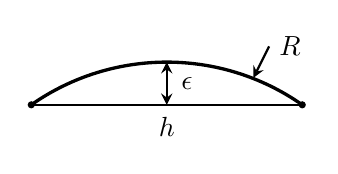
\begin{tikzpicture}[x=1cm,y=1cm,>=stealth]
    \def\Rc{3}
    \pgfmathsetmacro{\ang}{35}
    \pgfmathsetmacro{\xh}{\Rc*sin(\ang)}
    \pgfmathsetmacro{\yc}{-\Rc*(1-cos(\ang))}
    \draw[very thick] ({-\xh},\yc)
        arc[start angle={90+\ang}, end angle={90-\ang}, radius=\Rc];
    \draw[thick] ({-\xh},\yc) -- ({\xh},\yc);
    \fill ({-\xh},\yc) circle (1.3pt);
    \fill ({\xh},\yc) circle (1.3pt);
    \draw[<->,thick] (0,\yc) -- (0,0);
    \node[anchor=west] at (0.06,{0.5*\yc}) {$\sag$};
    \node[anchor=north] at (0,{\yc-0.03}) {$h$};
    \draw[->,thick] (1.3,0.2) node[anchor=west]{$\Rmink$} -- (1.1,-0.2);
  \end{tikzpicture}
  \end{minipage}\hfill
  \begin{minipage}{0.55\linewidth}
  \caption{Resolution control (2D). Across a rounded feature of radius $\Rmink$, a
  mesh edge of length $h$ (chord) leaves a sag $\sag\approx h^2/(8\Rmink)$ from the
  true surface (arc). A target sag $\sag$ therefore sets the grid step
  $h\approx\sqrt{8\,\sag\,\Rmink}$.}
  \label{fig:sag}
  \end{minipage}
\end{figure}

\paragraph{Resolution and tolerance} A single tolerance controls this error: the
target \emph{chordal error} $\sag$, or \emph{sag} (from \emph{sagitta}), the
largest gap between a mesh edge and the true surface (Figure~\ref{fig:sag}). It is
the option \code{epsilon} of \code{ShapeMeshOptions}, in the length unit of the
shape file; when it is zero, $\sag = \code{epsilonRel}\times\Rmink$ with
\code{epsilonRel}~$=0.01$. Across a rounded feature of radius $\Rmink$, a chord of
length $h$ gives $\sag\approx h^2/(8\Rmink)$, hence $h\approx\sqrt{8\,\sag\,\Rmink}$.
Since $\Rmink$ is the smallest radius of curvature of an $R$-shape, this step
resolves every rounded edge and corner with the same sag, and flat faces need no
finer step. The mesh is an inscribed polyhedron, so its volume converges to that
of the smooth solid as $\mathcal{O}(h^2)$, that is, linearly in $\sag$.

\paragraph{Mesh size and cost} The surface has about one triangle per area $h^2$,
so the number of triangles scales as $1/(\sag\Rmink)$. The computing time,
however, is dominated by the $\mathcal{O}\big((L/h)^3\big)$ grid nodes for a shape
of size $L$, while only $\mathcal{O}\big((L/h)^2\big)$ cells produce triangles.
Hence the need for fast queries and for a limit on the grid size.

\paragraph{Thin features and budget} A shape that is not a filled solid
(\code{isSolid()} false: sphere, capsule, plate, open surface) has a size of order
$\Rmink$ or is a slab of thickness $2\Rmink$; its step is limited to
$h\le\Rmink/2$ so that the grid does not step over it. A filled solid needs no such
limit. In addition, \code{maxCells} ($2\times10^7$ grid nodes by default) protects
against a large thin shape, such as a wall: when the requested step would exceed
it, $h$ is increased to fit and a message is printed.

\paragraph{Acceleration} Both queries (closest point, and ray where needed) use the
bounding-volume hierarchies of \code{ShapeSDF}, which reduce the search of
Equation~(\ref{eq:distmin}) from $\mathcal{O}(|\skel|)$ to about
$\mathcal{O}(\log|\skel|)$. The grid sampling runs on several threads with
OpenMP~\cite{dagum1998} when the code is compiled with it.

\paragraph{One mesh per shape} The mesh lives in the body frame and depends only on
the skeleton and the radius, not on the position or orientation of a particle.
Since \code{Shape::homothety()} scales both the vertices and $\Rmink$, two
homothetic shapes are similar and one mesh plus a scale factor describes both. A
sample of thousands of grains built from a few shapes needs only a few meshes,
which is what makes an explicit surface affordable for a whole scene.

\paragraph{Sharp reentrant edges} The Minkowski sum keeps reentrant edges sharp
(Section~\ref{sec:rshapes}), but marching cubes on a uniform grid rounds them over
a length of about $h$. This small visual effect is accepted. The positions and
normals already stored are the Hermite data used by extended marching
cubes~\cite{kobbelt2001} or dual contouring~\cite{ju2002}, which would recover the
crease.

% =====================================================================
\section{Coplanar simplification (\texttt{simplifyCoplanar})}
\label{sec:simplify}

Marching cubes cuts a flat region into many small coplanar triangles. On an
$R$-shape, the flat regions are the offset faces, which are exact planes, so their
triangulation can be made coarser without moving the surface. The function
\code{simplifyCoplanar(mesh, options)} (\code{src/Core/ShapeMeshSimplify.cpp})
does this, in the spirit of the coplanar merge of Hinker and
Hansen~\cite{hinker1993} and of superfaces~\cite{kalvin1996}: it removes the
interior vertices of planar regions and keeps their boundary unchanged. A general
decimation~\cite{schroeder1992,garland1997} would also coarsen these regions, but it
moves vertices and balances an error against a size; on an exactly planar region
the merge removes triangles with no geometric error.

\paragraph{Region growing} A region starts from a seed triangle and adds a
neighbour when its normal agrees with the seed normal within
\code{angleToleranceDeg} ($0.25^\circ$ by default) and each of its vertices lies
within a distance tolerance of the seed plane. The seed plane is fixed for the
whole region, so a chain of slightly tilted triangles cannot drift away from it.
On the offset faces both tests pass up to rounding, while curved patches are never
merged because neighbouring normals across a rounded edge differ by much more than
the angle tolerance.

\paragraph{The distance tolerance follows the mesh} This tolerance bounds how much
the surface can move when an interior vertex is removed. It is
\code{planeToleranceSag} times the sag of the mesh (one twentieth by default), so
the error of the merge is always a small fraction of the mesh error and decreases
with it. A tolerance tied to the bounding box, a natural first choice that was the
first implementation, stays fixed while the mesh error decreases and ends up being
the largest error (Section~\ref{sec:results}). \code{planeToleranceRel} is used only
for a mesh that carries no sag.

\paragraph{Re-triangulation} The boundary edges of a region, connected end to end,
form an oriented loop, which is triangulated in the region plane by ear
clipping~\cite{meisters1975,orourke1998}. Every boundary vertex must be kept: the
neighbouring curved regions are not modified and keep every vertex of the shared
boundary, and removing one would create a $T$-junction and break watertightness. A
flat face with $n$ boundary vertices then goes from $\mathcal{O}(n^2)$ grid
triangles to $n-2$ triangles. Keeping every boundary vertex makes the loop hard to
triangulate, because marching-cubes boundaries have long collinear runs, a known
difficulty of ear clipping on degenerate polygons~\cite{held2001}. Three measures
make it robust: the point-in-triangle test is \emph{strict}, so a vertex lying on
an edge of a candidate ear does not block it; among the valid ears the largest is
clipped first, so collinear points become the base of well-shaped triangles; and
every clipped triangle is checked to be empty. If no safe ear is left, or if the
boundary is not one simple loop (a face with a hole), the region keeps its original
triangles. Without these measures, the concave face of an L-shaped prism
(Figure~\ref{fig:reentrant}) was closed by a triangle across its notch.

\paragraph{Properties} The merge does not move or add any vertex and keeps every
boundary edge, so the mesh stays a closed two-manifold with the same Euler
characteristic, and a concave face is handled correctly. On an exactly planar
region it preserves the volume exactly; elsewhere, a thin strip of the
neighbouring rounded part may pass as flat, and the change is bounded by the
distance tolerance. The saving depends on how flat the surface is
(Figure~\ref{fig:simplify}): large for a rounded polyhedron, none for a sphere.

\begin{figure}[t]
  \centering
  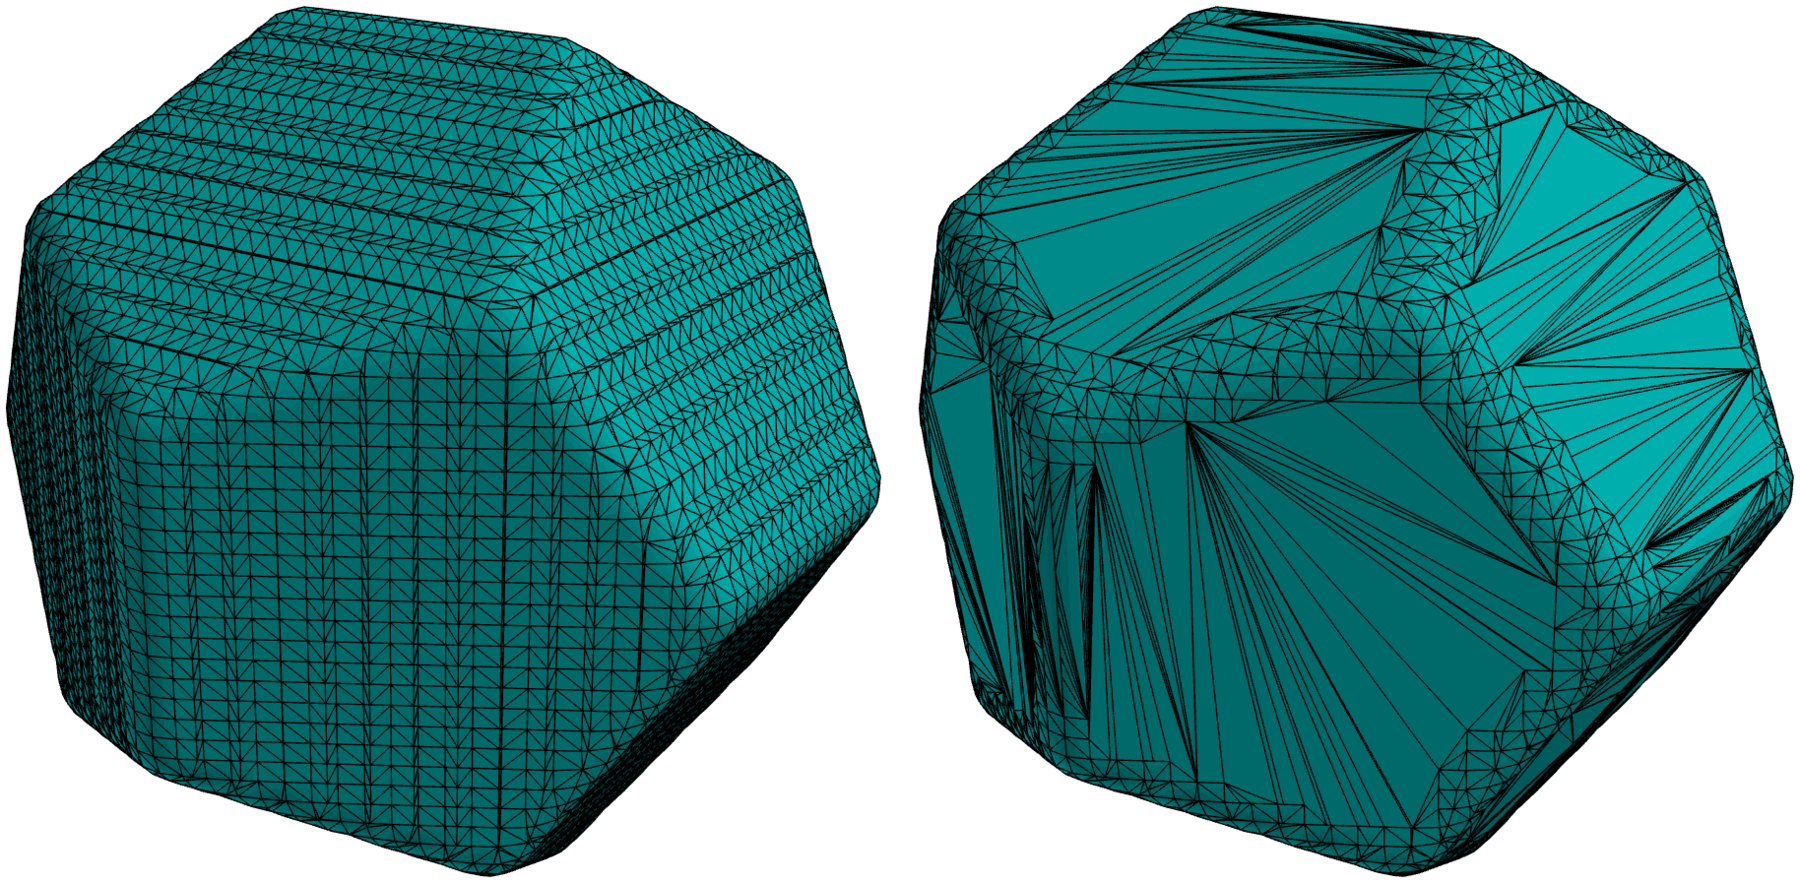
\includegraphics[width=0.8\linewidth]{figures/simplify}
  \caption{Coplanar simplification of a rounded polyhedron, drawn by the
  \code{Rockable} viewer. Left: the marching-cubes mesh ($15\,500$ triangles).
  Right: after \code{simplifyCoplanar} ($5\,840$ triangles); the flat offset faces
  are re-triangulated from their boundary, the rounded edges and corners keep
  their resolution, and the mesh stays watertight.}
  \label{fig:simplify}
\end{figure}

% =====================================================================
\section{Mass properties by the divergence theorem}
\label{sec:mass}

A DEM code needs the volume, centre of mass and inertia tensor of each grain. In
\code{Rockable}, \code{Shape::massProperties()} estimates them by quasi-Monte-Carlo
integration over the bounding box: the points come from a Sobol
sequence~\cite{sobol1967,niederreiter1992}, their number is set by the keyword
\code{MCnstep} of the shape file ($10^4$ by default, clamped to
$[10^3,10^7]$), and each point is tested with \code{Shape::inside()}. The results
are written back to the shape file (\code{volume}, \code{I/m}, \code{preCompDone});
\code{shapeSurvey -P} runs this computation without a window. The estimate is
cheap to write but its error decreases slowly and irregularly with the number of
samples, and the inertia tensor remains noisy. The watertight mesh gives a
deterministic alternative.

With the divergence theorem~\cite{lien1984,mirtich1996}, any volume integral over
the solid becomes a sum over the triangles. With $(\vect{a},\vect{b},\vect{c})$ the
vertices of triangle~$t$, $d_t=\vect{a}\cdot(\vect{b}\times\vect{c})$ and
$\vect{s}=\vect{a}+\vect{b}+\vect{c}$,
%
\begin{equation}
  V = \frac{1}{6}\sum_{t} d_t,
  \qquad
  V\vect{C}_g = \frac{1}{24}\sum_{t} d_t\,\vect{s},
  \qquad
  \int_{\shape}\!\vect{x} \vect{x}^{\mathsf{T}}\,\mathrm{d}V
    = \frac{1}{120}\sum_{t} d_t\big(\vect{a}\vect{a}^{\mathsf{T}}
      +\vect{b}\vect{b}^{\mathsf{T}}+\vect{c}\vect{c}^{\mathsf{T}}
      +\vect{s}\vect{s}^{\mathsf{T}}\big),
  \label{eq:meshmoments}
\end{equation}
%
which are the exact integrals over the tetrahedra joining the origin to each
triangle~\cite{tonon2005,kallay2006}. The inertia tensor about $\vect{C}_g$ follows
from the second-moment matrix with the parallel-axis theorem. These values are
exact for the meshed polyhedron and converge to those of the smooth solid as
$\mathcal{O}(h^2)$, linearly in~$\sag$.

\paragraph{State of the code} In the library, the volume and the area are
computed for every mesh by \code{ShapeMesh::computeVolume()} and
\code{computeArea()}, and stored in the fields \code{volume} and \code{area}. The
centre of mass and the inertia of Equation~(\ref{eq:meshmoments}) are, at the time
of writing, only implemented in the benchmark program used for
Figure~\ref{fig:divergence}; \code{Shape::massProperties()} still uses the Sobol
estimate. Moving these sums into the library, as an option of the pre-computation,
is the natural next step.

\paragraph{Comparison} Figure~\ref{fig:divergence} compares the two methods on a
capsule, the concave L-prism and the Stanford bunny, all with $\Rmink=2$~mm,
as the relative error versus computing time (Apple M4 laptop, 10 cores, GCC~16
with optimisation and OpenMP). A single Sobol run gives one fixed error that does
not decrease monotonically with~$N$; to measure the \emph{typical} error, the
sequence is randomised with a Cranley--Patterson shift~\cite{cranley1976}, and the
mean over independent replicates is plotted with their spread. The capsule has a
closed-form reference; for the L-prism and the bunny the reference is a Richardson
extrapolation~\cite{richardson1927} of the two finest meshes,
$V^{*}\approx V_{f}+(V_{f}-V_{c})/\big((h_{c}/h_{f})^{2}-1\big)$, done also for each
component of the centre of mass and inertia.

The Monte-Carlo error decreases roughly as $N^{-2/3}$. A heuristic argument
explains this: the integrand is an indicator function, so the error comes from the
cells of side $N^{-1/3}$ crossed by the surface, about $N^{2/3}$ of them, each
contributing an error of order $1/N$ with independent signs after the random
shift, hence $\sqrt{N^{2/3}}/N=N^{-2/3}$. Rigorous rates for randomised
quasi-Monte-Carlo on discontinuous integrands are given by He and
Wang~\cite{he2015}. One more decade of accuracy thus costs about three decades of
samples, whereas the divergence-theorem error decreases as the inverse of the
number of triangles. On the bunny, where each inclusion test casts a ray against
hundreds of faces, the best Monte-Carlo point reaches $1.1\times10^{-4}$ in
$34$~s, while the triangle sum reaches it in $1.6$~ms once the mesh exists, and in
$9$~s including the mesh build.

For the inertia tensor (error measured with the Frobenius norm), the mesh values
keep the second order (measured order $2.0$ on the three shapes) and the error is
$1.4$ to $2.3$ times the volume error at the finest mesh, whereas the Monte-Carlo
inertia error is two to three times its volume error, since the second moments
weight each sample by a squared distance. At the finest meshes (four to ten million
triangles, a few tens of milliseconds per sum), the relative volume errors are
$3.9\times10^{-6}$ (capsule), $4.9\times10^{-6}$ (L-prism) and $6.2\times10^{-6}$
(bunny), and the centre of mass is within $3\times10^{-9}$, $2\times10^{-7}$ and
$6\times10^{-7}$ of the reference, in units of the shape size.

\begin{figure}[t]
  \centering
  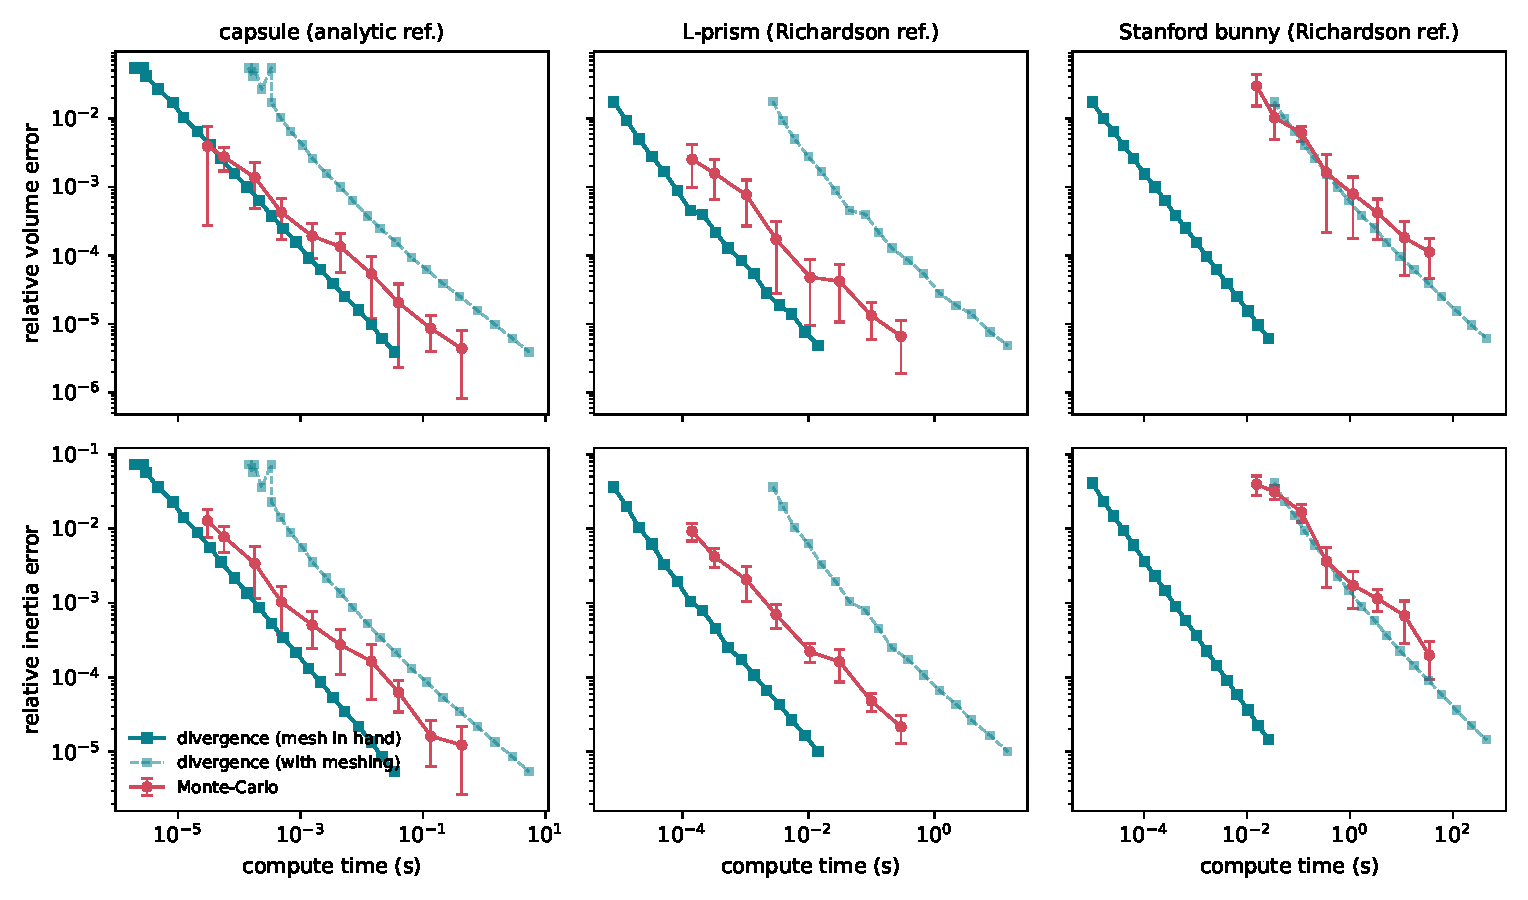
\includegraphics[width=\linewidth]{figures/convergence}
  \caption{Mass properties by quasi-Monte-Carlo (the Sobol estimator of
  \code{Shape::massProperties()}) versus the divergence theorem on the skin mesh,
  for three $R$-shapes at $\Rmink=2$~mm: relative errors of the volume (top) and
  of the inertia tensor (bottom, Frobenius norm) versus computing time.
  Monte-Carlo (red): mean over randomised-Sobol replicates, with their spread.
  Divergence theorem: solid line with the mesh already built, dashed line including
  the mesh build. Reference: analytic for the capsule, Richardson extrapolation
  otherwise; points within three times the uncertainty of the reference
  ($1.2\times10^{-6}$ for the L-prism, $3.3\times10^{-7}$ for the bunny) are not
  plotted. The reentrant crease of the L-prism adds an error term not cancelled by
  the pure $h^2$ extrapolation.}
  \label{fig:divergence}
\end{figure}

\paragraph{Refinement as a diagnostic} The convergence is also a test of the
\emph{input}. As downloaded, the bunny skeleton has two vertices
$7.4\times10^{-5}$~m apart ($3.7\%$ of $\Rmink$) that were never merged. This pair
creates a degenerate face and two dangling edges, so the faces are not a closed
manifold and the sign falls back to ray casting; a ray leaving through the
degenerate face counts one crossing too many, so a region of fixed size gets the
wrong sign. Figure~\ref{fig:defect} shows that the two series agree down to a
relative error of about $10^{-4}$, after which the imported skeleton stops
converging while the repaired one keeps decreasing. Such a defect is invisible in a
viewer and in a coarse mass computation. It is revealed by meshing at two
resolutions and comparing the volumes, and the choice of the sign rule already
flags it: a closed-looking shape that falls back to ray casting has faces that are
not a clean manifold and deserves a check.

\begin{figure}[tb]
  \centering
  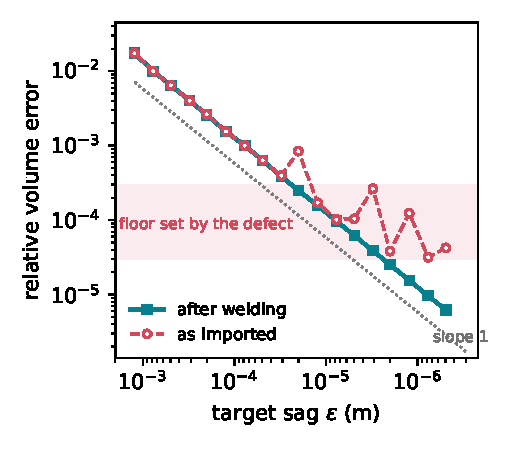
\includegraphics[width=0.6\linewidth]{figures/defect}
  \caption{Effect of one duplicate vertex: relative error of the skin-mesh volume
  of the Stanford bunny versus the target sag, for the file as imported (circles)
  and after merging its duplicate vertex (squares). Below about $10^{-4}$, the
  imported skeleton stops converging (shaded band), while the repaired one keeps
  decreasing at order one in the sag (dotted line).}
  \label{fig:defect}
\end{figure}

\paragraph{Oriented bounding box} The mesh could also serve the oriented bounding
box used for neighbour detection. \code{Rockable} fits its orientation on the
skeleton vertices only (option \code{fibObbOption}) and enlarges the box by
$\Rmink$; a skeleton with few vertices (a capsule has two) gives little
information, whereas the mesh vertices sample the real surface evenly. This is left
for future work.

% =====================================================================
\section{Tools and files}
\label{sec:usage}

The tools of Sections~\ref{sec:sdf}--\ref{sec:mass} belong to the C++ core library
of \code{Rockable} (target \code{Rockable\_core}), distributed under the CeCILL-B
licence, with no external dependency beyond the optional OpenMP already used by
the DEM code. All functions work in the body frame and do not modify the shape.
Table~\ref{tab:codemap} maps the sections of this note to the code.

\begin{table}[tb]
  \centering
  \small
  \caption{Where each part of this note lives in the code.}
  \label{tab:codemap}
  \begin{tabularx}{\linewidth}{@{}l>{\raggedright\arraybackslash}X>{\raggedright\arraybackslash}X@{}}
    \toprule
    Section & Code & File \\
    \midrule
    \ref{sec:rshapes} $R$-shape & \code{Shape}, \code{Shape::inside()} & \code{src/Core/Shape.hpp} \\
    \ref{sec:sdf} SDF and sign & \code{ShapeSDF}: \code{closestPoint}, \code{value},
      \code{gradient}, \code{inside}, \code{isClosedVolume}, \code{isSolid},
      \code{skeletonVolume} & \code{src/Core/ShapeSDF.hpp/.cpp} \\
    \ref{sec:meshing} Meshing & \code{buildShapeMesh}, \code{ShapeMeshOptions}
      (\code{epsilon}, \code{epsilonRel}, \code{newtonIters}, \code{marginCells},
      \code{maxCells}), \code{ShapeMesh} & \code{src/Core/ShapeMesh.hpp/.cpp} \\
    \ref{sec:simplify} Merge & \code{simplifyCoplanar}, \code{SimplifyOptions}
      (\code{angleToleranceDeg}, \code{planeToleranceSag}, \code{planeToleranceRel})
      & \code{src/Core/ShapeMeshSimplify.cpp} \\
    \ref{sec:mass} Mass & \code{ShapeMesh::computeVolume}, \code{computeArea};
      Monte-Carlo: \code{Shape::massProperties}, keyword \code{MCnstep}
      & \code{src/Core/ShapeMesh.cpp}, \code{src/Core/Shape.cpp} \\
    \ref{sec:usage} Export & \code{writeOBJ}, \code{writePLY}, \code{writeRmsh},
      \code{loadRmsh} & \code{src/Core/ShapeMesh.cpp} \\
    \ref{sec:usage} Mesher & \code{shape2mesh} & \code{prepro/converters/shape2mesh/} \\
    \ref{sec:usage} Viewers & \code{see} (reads \code{<stem>.rmsh}),
      \code{shapeSurvey --skin} & \code{src/Apps/see.cpp},
      \code{prepro/shapesurvey/} \\
    \ref{sec:results} Tests & \code{test\_ShapeSDF}, \code{test\_ShapeMesh}
      (\code{ctest -R Shape}) & \code{test/ShapeSDF/} \\
    \bottomrule
  \end{tabularx}
\end{table}

\paragraph{Command-line mesher} \code{shape2mesh} applies these functions to a
shape file:
{\small
\begin{verbatim}
shape2mesh shapes.txt -f ply -e 1e-3 -s     # one PLY per shape, sag 1e-3, merged
shape2mesh shapes.txt --rmsh -s             # all shapes -> shapes.rmsh, for the viewer
\end{verbatim}
}
\noindent The options are \code{-f obj|ply} (format), \code{-e} (sag, in the length
unit of the shape file; default $1\%$ of~$\Rmink$), \code{-s [deg]} (coplanar merge,
with an optional angle tolerance), \code{-r}/\code{--rmsh} (companion file) and
\code{-o} (output directory). OBJ and PLY files carry the exact normals as vertex
normals and can be opened in Blender, MeshLab or ParaView. A file with one shape
gives \code{<stem>.<ext>}, a file with several shapes
\code{<stem>\_<shapeName>.<ext>}. In \code{--rmsh} mode without \code{-e}, each
shape gets its own sag, $0.4\%$ of the diagonal of its bounding box, so that a large
wall and a small grain in the same file both get a suitable mesh.

\paragraph{Companion mesh file} A \code{.rmsh} file stores the skin mesh of each
shape as one block named after the shape (positions, exact normals, triangles).
When \code{see} opens a configuration, it looks for a file with the base name of
the shape file and the extension \code{.rmsh}; the mesh of each shape found there is
compiled once into an OpenGL display list and drawn for every particle of this
shape with its position, orientation and homothety applied. Shapes without a block,
and soft particles, are drawn with the overlapping primitives. The simulation files
are not modified, and the meshing cost is paid once, before visualisation.

\paragraph{Shape viewer} \code{shapeSurvey} draws a skin with
\code{--skin file.rmsh}, and has a screenshot mode (\code{-o file.png}, with
\code{--elev}, \code{--azim}, \code{-A} for the opacity, \code{--wire},
\code{--radius} to override $\Rmink$) that renders a single frame and exits. All
renderings of this note were produced this way.

\paragraph{Typical workflow}
\begin{enumerate}[nosep]
  \item Build or import the shapes (\code{stl2shape} for an STL), check them in
    \code{shapeSurvey}, and pre-compute them once with
    \code{shapeSurvey shapes.txt -P shapes.txt}. A shape still marked
    \code{preCompDone n} is otherwise pre-computed by \code{shape2mesh} itself at
    each run, with the Monte-Carlo cost of Section~\ref{sec:mass}, because the
    mesh is built in the body frame (mass centre and principal axes).
  \item Run \code{shape2mesh shapes.txt --rmsh -s} next to the shape file.
  \item Open the configuration in \code{see}: the console reports
    \emph{``Loaded $n$ skin mesh(es) from shapes.rmsh''}.
  \item Re-run step 2 whenever a shape changes: the \code{.rmsh} file is a cache and
    is not updated automatically.
\end{enumerate}

\paragraph{Choosing the sag} The default sags are meant for display. For export
or for mass properties, a sag of $10^{-3}\Rmink$ to $10^{-2}\Rmink$ is typical;
halving it roughly doubles the number of triangles. If \code{shape2mesh} reports
that the grid budget was reached, the shape is large compared with $\Rmink$ (a
wall): increase the sag for this shape, or raise \code{maxCells} in a program
linked to the library.

% =====================================================================
\section{Validation}
\label{sec:results}

The two test programs of \code{test/ShapeSDF} (\code{test\_ShapeSDF} and
\code{test\_ShapeMesh}, registered in CTest as \code{ShapeSDF} and \code{ShapeMesh})
check the properties below, on shapes whose distance function is known in closed
form, against the Monte-Carlo volume of \code{Shape::massProperties()}, and on real
shapes, including a model imported from an STL file (Figure~\ref{fig:gallery}).

\begin{figure}[t]
  \centering
  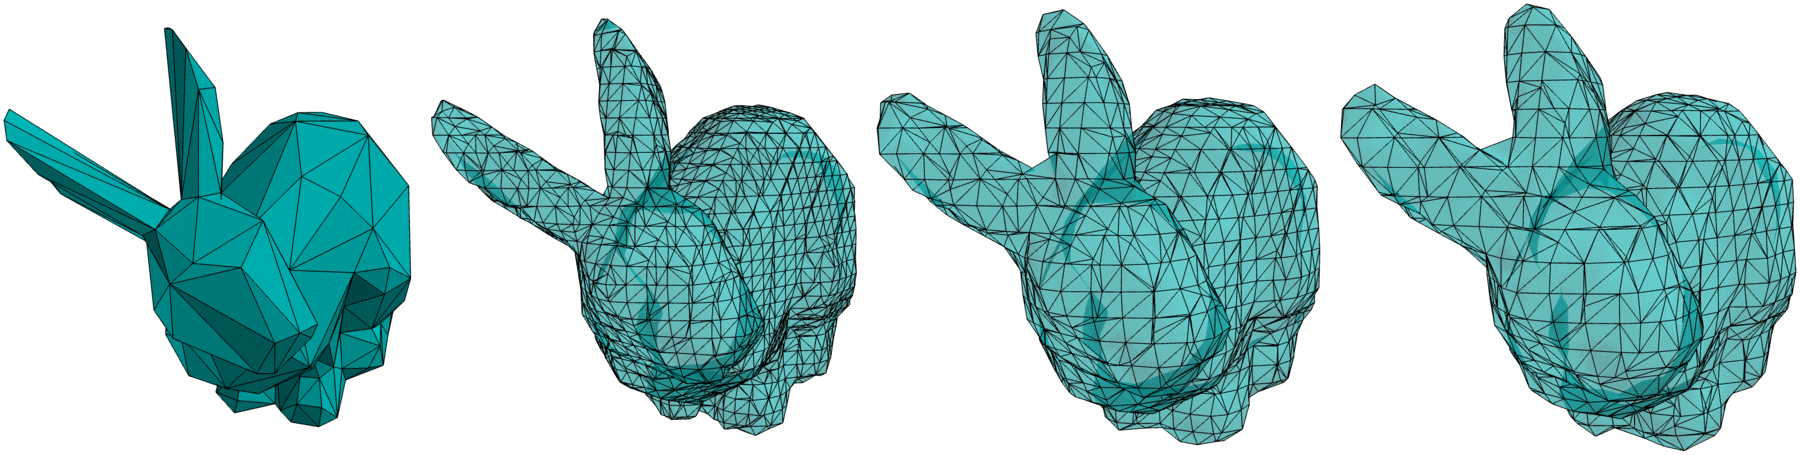
\includegraphics[width=\linewidth]{figures/gallery}
  \caption{An STL imported as an $R$-shape (\code{stl2shape}), drawn by the viewer
  with the mesh wireframe. The triangles become the skeleton, to which a radius is
  given. From left to right, the Stanford bunny (about $100$~mm long) with
  $\Rmink=0$, $2$, $4$ and $5$~mm; the panels with $\Rmink>0$ show the skin mesh.}
  \label{fig:gallery}
\end{figure}

\paragraph{Distance and normals} A sphere, a capsule, a rounded box and a plate
have hand-written SDFs. Over $2\times10^4$ random points, \code{ShapeSDF::value}
equals the closed form exactly for the first three and within
$2.2\times10^{-16}$ for the plate; $\big|\norm{\nabla\sdf}-1\big|\le3.3\times10^{-16}$
on all four, and the gradient agrees with a centred finite difference to
$3\times10^{-10}$, the accuracy of the finite difference. On closed skeletons, the
sign agrees with \code{Shape::inside()} at every sampled point.

\paragraph{Watertightness and surface accuracy} Every mesh is watertight (each edge
belongs to exactly two triangles), with Euler characteristic $\chi=2$ on the
sphere, capsule, rounded box, concave L and a rounded polyhedron. After the Newton
projection, $\max|\sdf|\approx5.6\times10^{-17}$ at the vertices of the polyhedron,
and the stored normals equal the analytic gradient.

\paragraph{Volume convergence} Over three grids with $h$ halved at each level, the
observed order is $1.96$ (sphere), $2.04$ (capsule) and $1.99$ (rounded box), and
$2.39$ for the concave L, whose rounded reentrant crease adds an error that
decreases faster. The limit is the true volume, as confirmed against the analytic
capsule and the Monte-Carlo estimate. This check also revealed that the volume
stored in one of the sample shape files did not match its own skeleton and radius.

\paragraph{Coplanar merge} After \code{simplifyCoplanar} the mesh is still
watertight with $\chi=2$, including the concave L. The number of triangles goes from
$15\,500$ to $5\,840$ ($-62\%$) on the rounded polyhedron and from $13\,716$ to
$6\,828$ ($-50\%$) on the L; a sphere is unchanged. With the tolerance tied to the
sag, the relative change in volume stays between $3\times10^{-7}$ and
$1\times10^{-6}$ on the polyhedron for sags from $4\times10^{-3}$ down to
$3\times10^{-4}$, while the saving grows from $52\%$ to $69\%$. With a tolerance
tied to the bounding box, the change \emph{grows} from $4\times10^{-6}$ to
$2\times10^{-5}$ over the same range, and would end up larger than the
discretisation error.

\paragraph{Performance} For a rock in the shape of a hand imported from an STL file
with about $2800$ faces, the direct $\mathcal{O}(|\skel|)$ search at every grid node
is impractical, while the hierarchy makes it routine: with OpenMP, a set of four
shapes including this model is meshed in about $16$~s, and the $309$-face bunny in
about $0.1$~s.

% =====================================================================
\section{Stress tests on very complex shapes}
\label{sec:complex}

The skeletons accepted by \code{Rockable} are not limited to rounded polyhedra:
faces may or may not enclose a volume, edges may have no face, a shape may combine
the three kinds of primitive, and through-openings or knots are allowed. The
mesher was tested on shapes built for this purpose, each with one kind of
complexity, and every mesh was checked for watertightness and topology: number of
connected components and Euler characteristic $\chi$ of each (vertices minus
edges plus triangles). A closed surface with no hole has $\chi=2$, and each
through-hole (handle) reduces $\chi$ by two: a torus has $\chi=0$, and $\chi=-8$
means genus~5.

\begin{figure}[t]
  \centering
  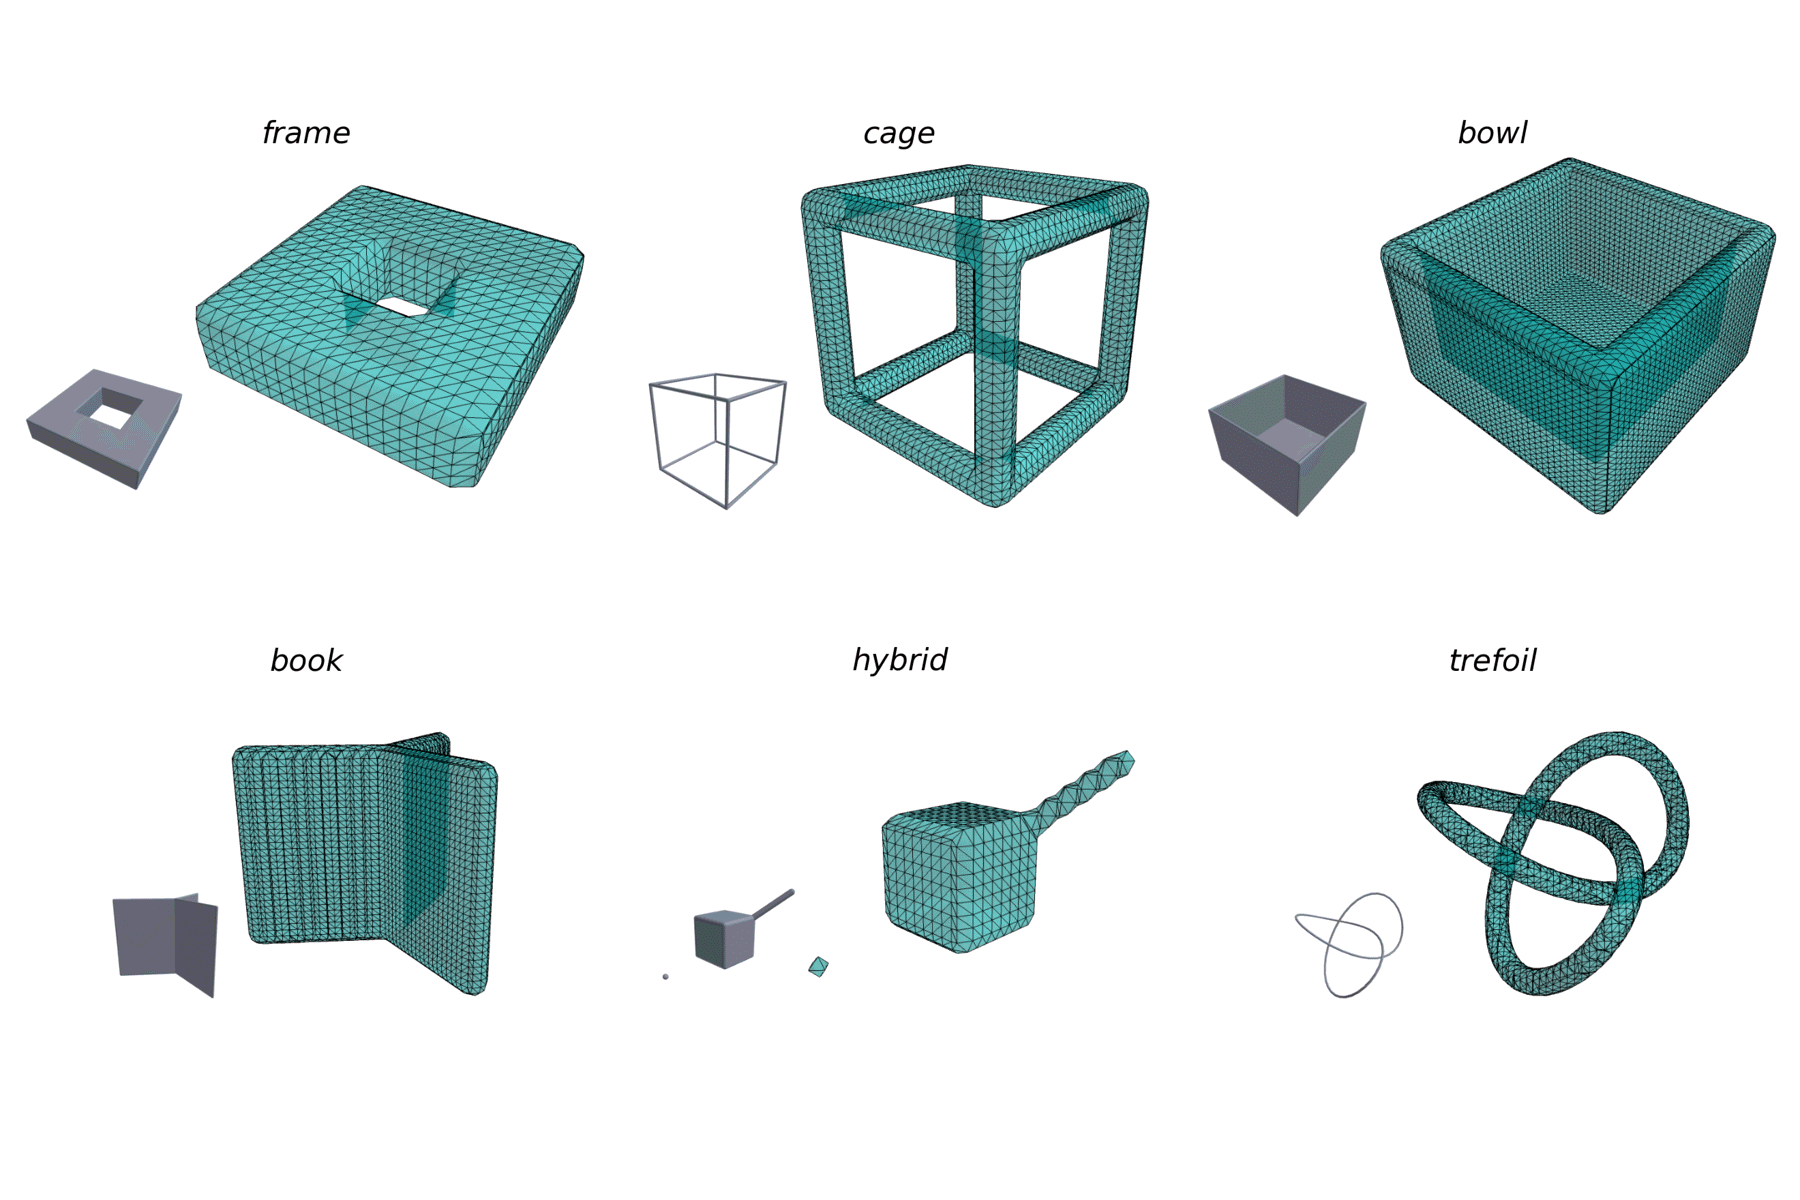
\includegraphics[width=\linewidth]{figures/complex-gallery}
  \caption{Six complex $R$-shapes and their skin meshes, drawn semi-transparently
  with the wireframe; next to each, in grey, its skeleton drawn with a small
  radius. Top: a \emph{frame} (genus-1 solid); a \emph{cage}, the twelve edges of a
  cube with no face (genus 5); a \emph{bowl}, a box without its lid declared as a
  surface (slab of thickness $2\Rmink$). Bottom: a \emph{book}, with one spine edge
  shared by three sheets (non-manifold); a \emph{hybrid}, a filled box with a
  dangling edge and an isolated vertex (two shells); a \emph{trefoil}, seventy-two
  capsules forming a knotted torus. Every mesh is watertight with the expected
  components and Euler characteristic.}
  \label{fig:complex-gallery}
\end{figure}

Figure~\ref{fig:complex-gallery} shows these shapes. The \emph{frame} keeps its
through-opening after dilation ($\chi=0$). The \emph{cage} is a union of capsules
joined at the eight corners, a genus-5 surface, and the mesh gives exactly
$\chi=-8$. The \emph{bowl} gives one watertight shell with a rounded rim ($\chi=2$).
The three slabs of the \emph{book} are joined along the spine into a single
watertight surface. The \emph{hybrid} gives the two expected shells (the box with
its tube, and the isolated ball), and the \emph{trefoil} a knotted torus with
$\chi=0$.

\begin{figure}[t]
  \centering
  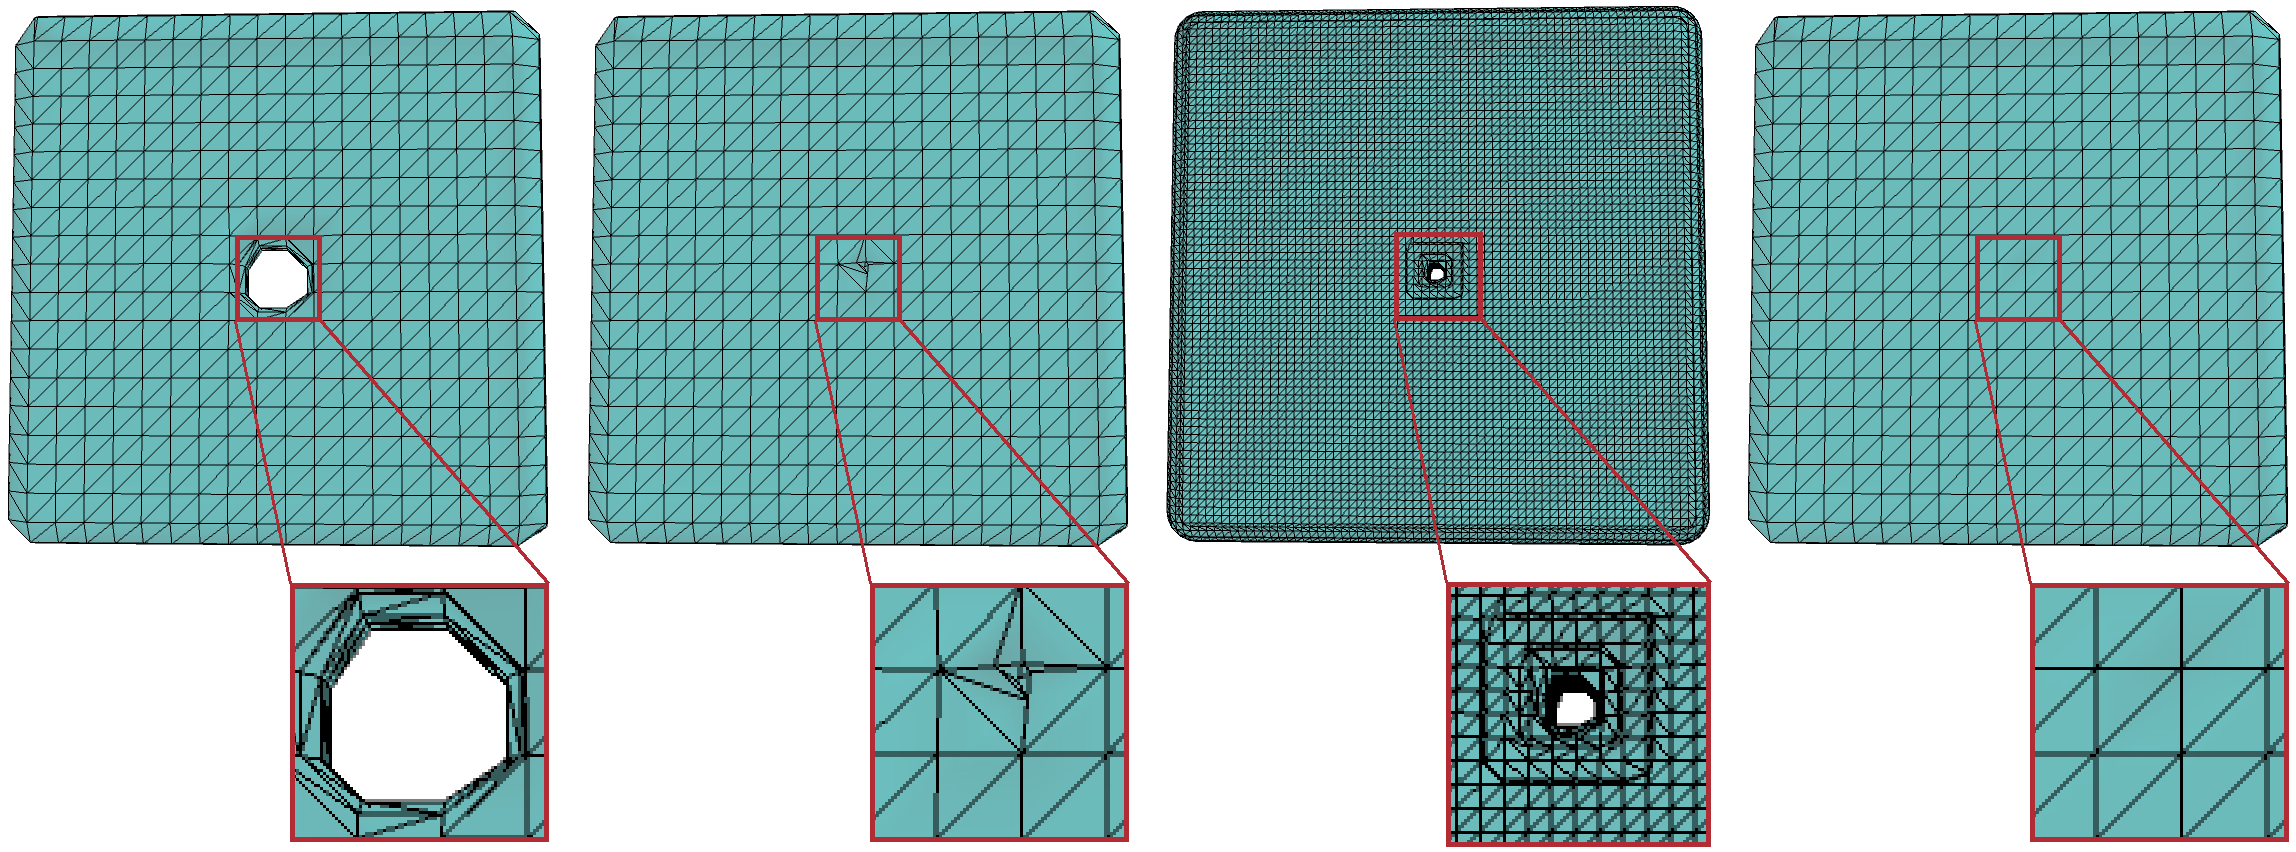
\includegraphics[width=\linewidth]{figures/plate-holes}
  \caption{A plate with a square through-hole of side $d$, seen from above, with
  the central region magnified (white seen through means the channel is open).
  From left to right: $d=4\Rmink$, the hole is kept (genus 1); $d=2.5\Rmink$ with
  the default sag, the remaining channel of width $\Rmink/2$ is smaller than the
  grid step and is closed, a failure invisible in a watertight mesh; the same with
  a finer sag, the hole is open again; $d=1.5\Rmink<2\Rmink$, the dilation itself
  fills the hole, and genus 0 is correct.}
  \label{fig:plate-holes}
\end{figure}

\paragraph{Thin openings} The dilation reduces a hole of width $d$ to $d-2\Rmink$
(Figure~\ref{fig:plate-holes}). For $d=4\Rmink$ the channel is $2\Rmink$ wide and
the genus is kept; for $d=1.5\Rmink$ the dilation fills the hole, which is the true
Minkowski geometry. For $d=2.5\Rmink$ the channel exists but is only $\Rmink/2$ wide,
smaller than the default step: no grid point falls inside it, marching cubes closes
it, and the mesh is still perfectly watertight, so nothing looks broken although
the genus is wrong. A finer sag gives the hole back.

\begin{figure}[tb]
  \centering
  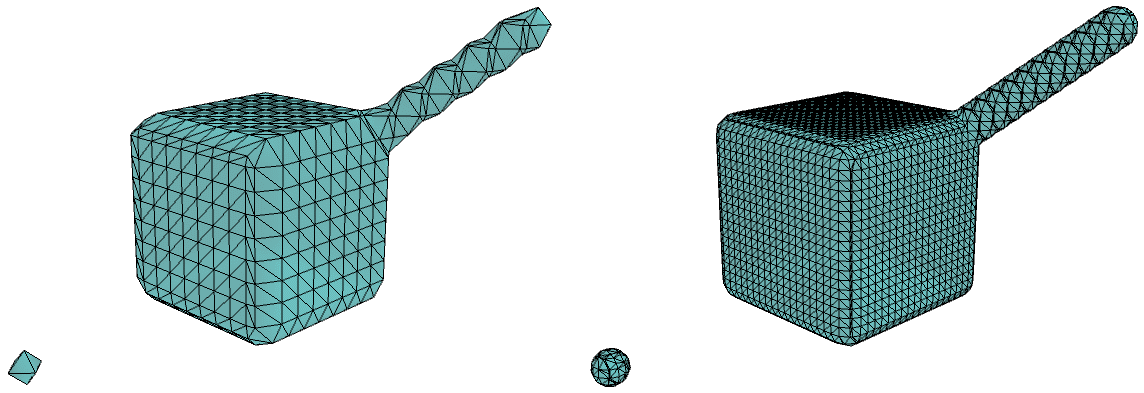
\includegraphics[width=0.6\linewidth]{figures/hybrid-pair}
  \caption{The hybrid at the default sag (left) and at a finer one (right). The
  shape is a filled solid, so the limit $h\le\Rmink/2$ does not apply, and the
  isolated ball and the tube are coarse at the default sag, with the correct
  topology.}
  \label{fig:hybrid-pair}
\end{figure}

\paragraph{Thin details on a solid} The hybrid \emph{is} a filled solid, so the
limit $h\le\Rmink/2$ of Section~\ref{sec:meshing} does not apply and its two
details of size $\Rmink$ are sampled with a step chosen for the box: the isolated
ball is reduced to a few triangles and the tube is irregular
(Figure~\ref{fig:hybrid-pair}), with a correct topology. A finer sag solves it.

\paragraph{Lessons} Every observed failure is topological; the mesh never has a
crack, because shared grid edges always give a watertight surface. Both failures
have the same cause, a feature (solid or empty) narrower than the grid step, and
the same remedy, a smaller sag. Thin solids are protected automatically, thin
openings are left to the user; a step limit based on the narrowest opening of the
skeleton would be the natural extension. Finally, the topology check is useful
beyond testing: the shape readers do not validate their input, and a shape
generator bug that produced an edge pointing to a non-existent vertex was read
without warning but immediately detected by the component and Euler-characteristic
check of its skin. This check is a cheap test for any imported shape.

% =====================================================================
\section{Summary and perspectives}
\label{sec:conclusion}

Because an $R$-shape is a Minkowski sum, its signed distance is the signed
distance to its skeleton minus the rounding radius, an exact function with an
analytic gradient. \code{Rockable} uses it, through \code{ShapeSDF}, to build a
watertight skin mesh by marching cubes and Newton projection
(\code{buildShapeMesh}), controlled by a single sag tolerance and accelerated by a
bounding-volume hierarchy; to remove the unneeded triangles of the flat faces
(\code{simplifyCoplanar}); and to obtain the mass properties by the divergence
theorem, deterministically and at second order, orders of magnitude faster than
the Sobol estimate for a given accuracy once the mesh exists. The sign rule handles
clean manifolds, imported meshes with defects, and open surfaces. The meshes are
written by \code{shape2mesh}, either as OBJ/PLY files or as a \code{.rmsh}
companion read by \code{see} and \code{shapeSurvey}.

The main purpose is visualisation: an explicit watertight surface can be shaded,
made transparent, lit with shadows and exported, which the overlapping primitives
cannot. Possible extensions are: computing the centre of mass and inertia from the
mesh inside \code{Shape::massProperties()}; recovering sharp reentrant
edges with extended marching cubes or dual contouring~\cite{kobbelt2001,ju2002}
from the data already stored; storing several levels of detail per shape for the
instanced rendering of large samples; extending the step limit to thin openings;
and using Steiner's formula, Equation~(\ref{eq:steiner}), as an exact reference
for convex shapes. The same steps (marching cubes, projection onto the zero level
set, moments by the divergence theorem) also apply to level-set
grains~\cite{kawamoto2016,kawamoto2018}, with a sampled rather than exact distance.

\paragraph{Note on the preparation} The geometric tools described here, the
companion mesh file, the viewer support and the benchmark scripts were written with
the help of an AI coding assistant (Anthropic's Claude, through Claude Code), which
was also used to draft and edit this note. The \code{Rockable} framework, its shape
model and its numerical methods predate this work. The author defined the goals,
reviewed every change and checked every reported number; several defects found
during this review (faces drawn inside a solid, a merge that closed a reentrant
notch, a tolerance that did not decrease with the mesh) are described in the text
with their correction. Every image is a rendering by the \code{Rockable} viewers or
a plot of computed data.

\small
\bibliographystyle{unsrtnat}
\bibliography{skin-meshes}

\end{document}
